\section{Background modeling}
\label{sec:BkgModeling}

\subsection{Blind strategy}
\label{subsec:BlindStrategy}
In the following sections, the modeling of kinematic distributions, particularly those used for BDT training, of the $t\bar{t}+\text{jets}$ background is checked by comparing the data and MC. In order to avoid observing signals or any other biases before fixing the analysis procedure, the following blinding strategy is applied. The signal-to-noise ratio ($S/B$) is calculated in each bin of each distribution for all mass hypotheses (more details in Appendix \ref{app:SignalBackgroundComparison}). The signal cross section (${\sigma}_{\text{signal}}$) on each mass hypothesis is set to 0.046 pb, which is the upper limit at 1 TeV $H^{+}$ mass point obtained from the resolved $H^{+}{\rightarrow}tb$ search \cite{HDBS-2021-02}. Therefore, it can be considered the most conservative assumption. The data in bins with $S/B>0.05$ in at least one mass hypothesis are blinded when the data is compared with MC.

\subsection{Data/MC comparison for BDT input variables}
\label{subsec:Data/MCBDTInputBeforeReweight}
Figures \ref{fig:DATAOVERMC_BDTInputs_Prefit} show the distributions of input variables for BDT training in the inclusive SR region (i.e., SR1+SR2). Data are blinded according to the blind strategy in Section \ref{subsec:BlindStrategy}. No significant difference between the data and MC is found in each variable.

\begin{figure}[H]
    \subfloat[HT\_jets] {
        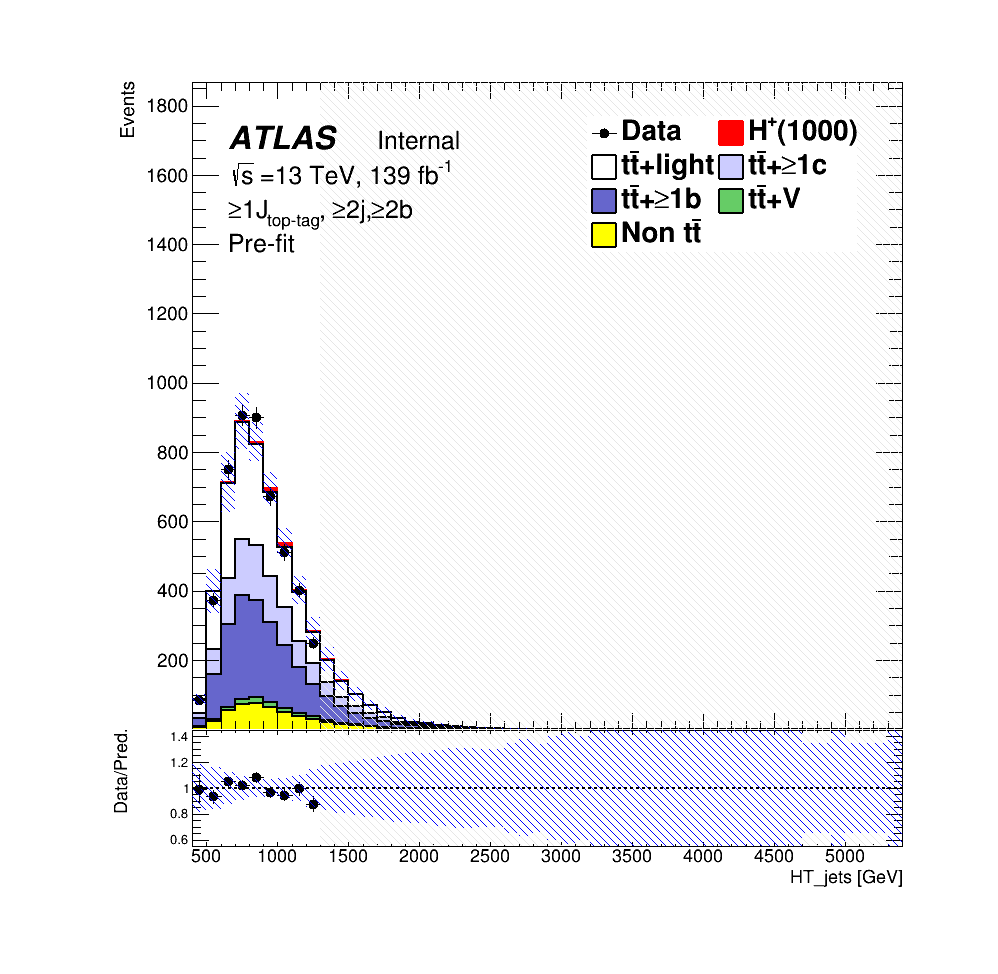
\includegraphics[width=0.50\textwidth]{images/BkgModeling/DATAOVERMC_Hp1000_Contained80_DL1r_70_HTjets_beforeRW_geq1tgeq2jgeq2b_prefit.png}
        \label{fig:DATAOVERMC_HT_jets}
    }
    \subfloat[LeadingJet\_pt] {
        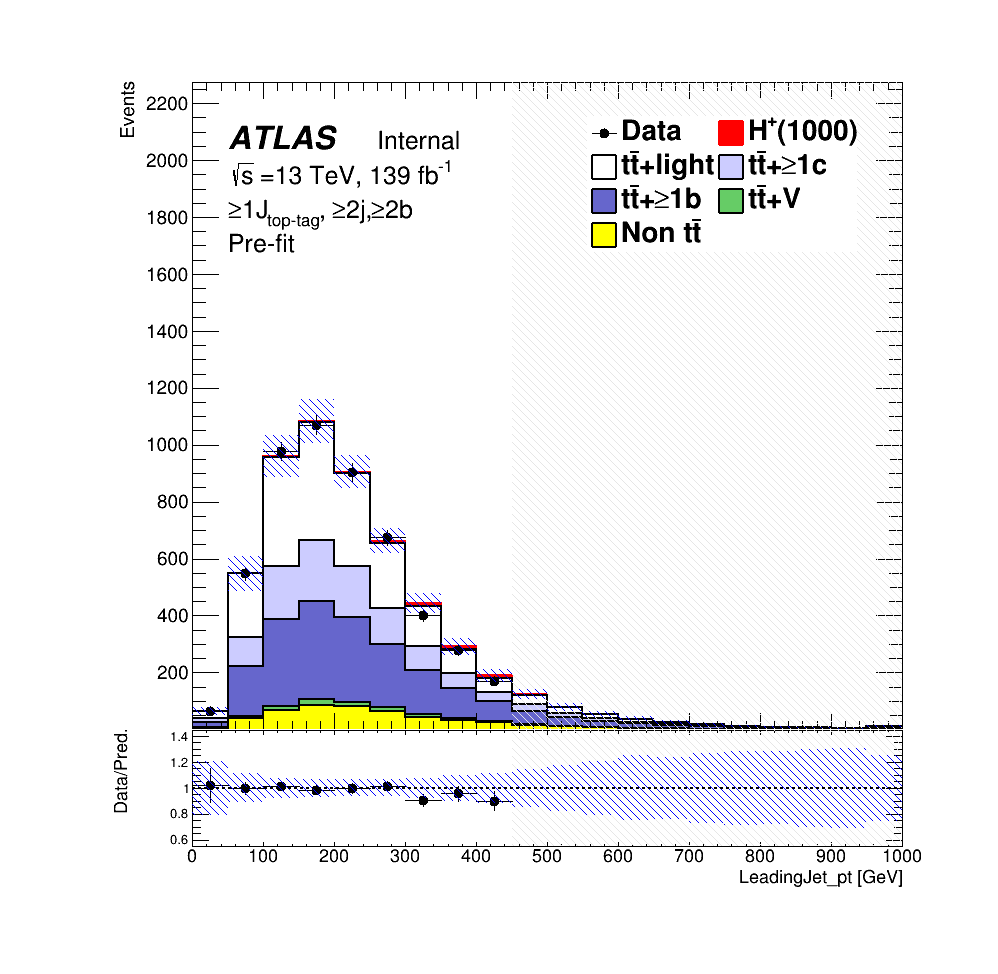
\includegraphics[width=0.50\textwidth]{images/BkgModeling/DATAOVERMC_Hp1000_Contained80_DL1r_70_LeadingJet_pt_beforeRW_geq1tgeq2jgeq2b_prefit.png}
        \label{fig:DATAOVERMC_LeadingJet_pt}
    }
\end{figure}
\begin{figure}[H]
    \addtocounter{figure}{-1}
    \subfloat[Centrality\_all] {
        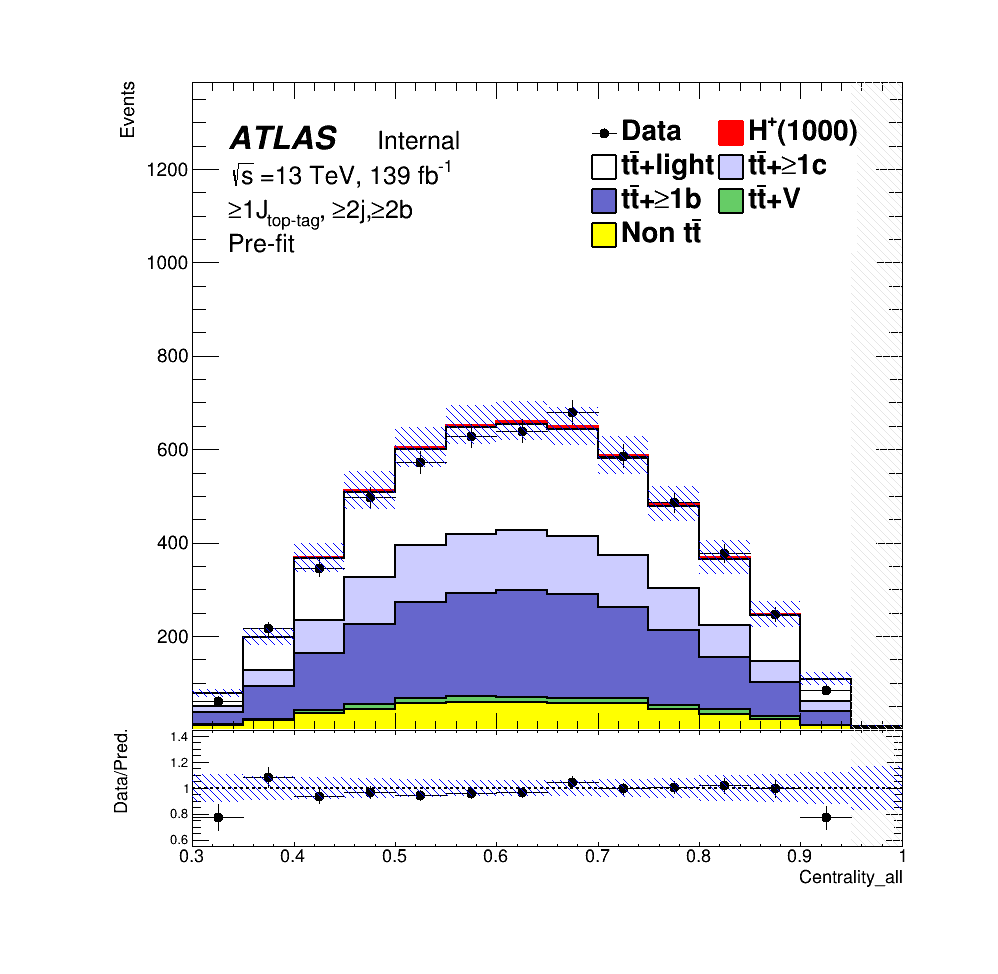
\includegraphics[width=0.50\textwidth]{images/BkgModeling/DATAOVERMC_Hp1000_Contained80_DL1r_70_Centrality_all_beforeRW_geq1tgeq2jgeq2b_prefit.png}
        \label{fig:DATAOVERMC_Centrality_all}
    }
    \subfloat[H1\_all] {
        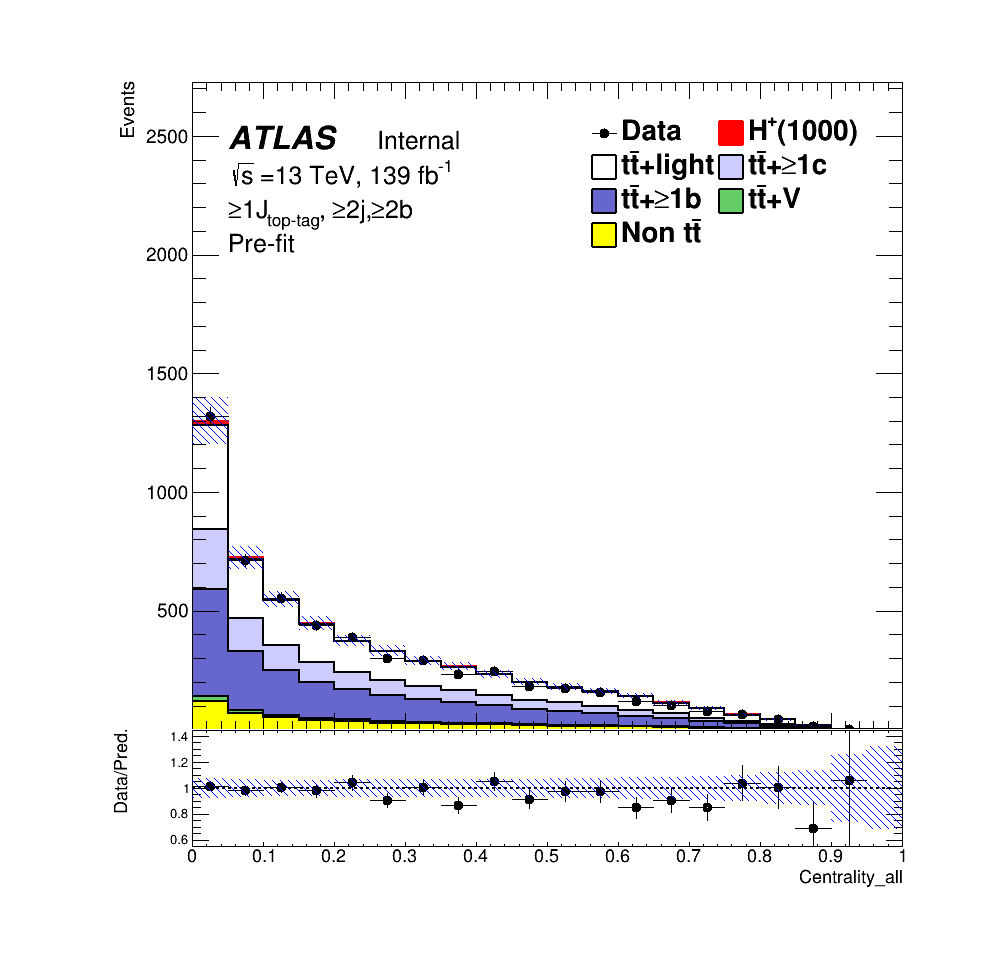
\includegraphics[width=0.50\textwidth]{images/BkgModeling/DATAOVERMC_Hp1000_Contained80_DL1r_70_H1_all_beforeRW_geq1tgeq2jgeq2b_prefit.png}
        \label{fig:DATAOVERMC_H1_all}
    }
\end{figure}
\begin{figure}[H]
    \addtocounter{figure}{-1}
    \subfloat[Mbb\_MaxPt] {
        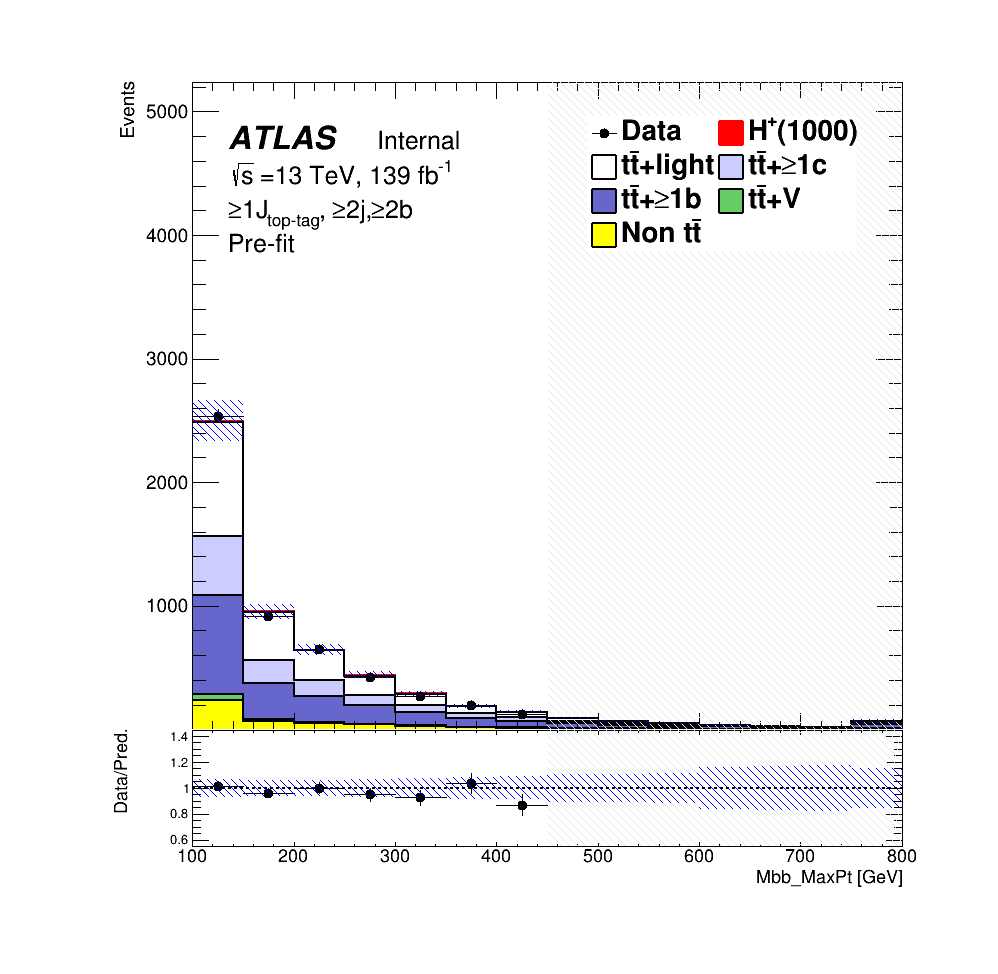
\includegraphics[width=0.50\textwidth]{images/BkgModeling/DATAOVERMC_Hp1000_Contained80_DL1r_70_Mbb_MaxPt_beforeRW_geq1tgeq2jgeq2b_prefit.png}
        \label{fig:DATAOVERMC_Mbb_MaxPt}
    }
    \subfloat[Mjjj\_MaxPt] {
        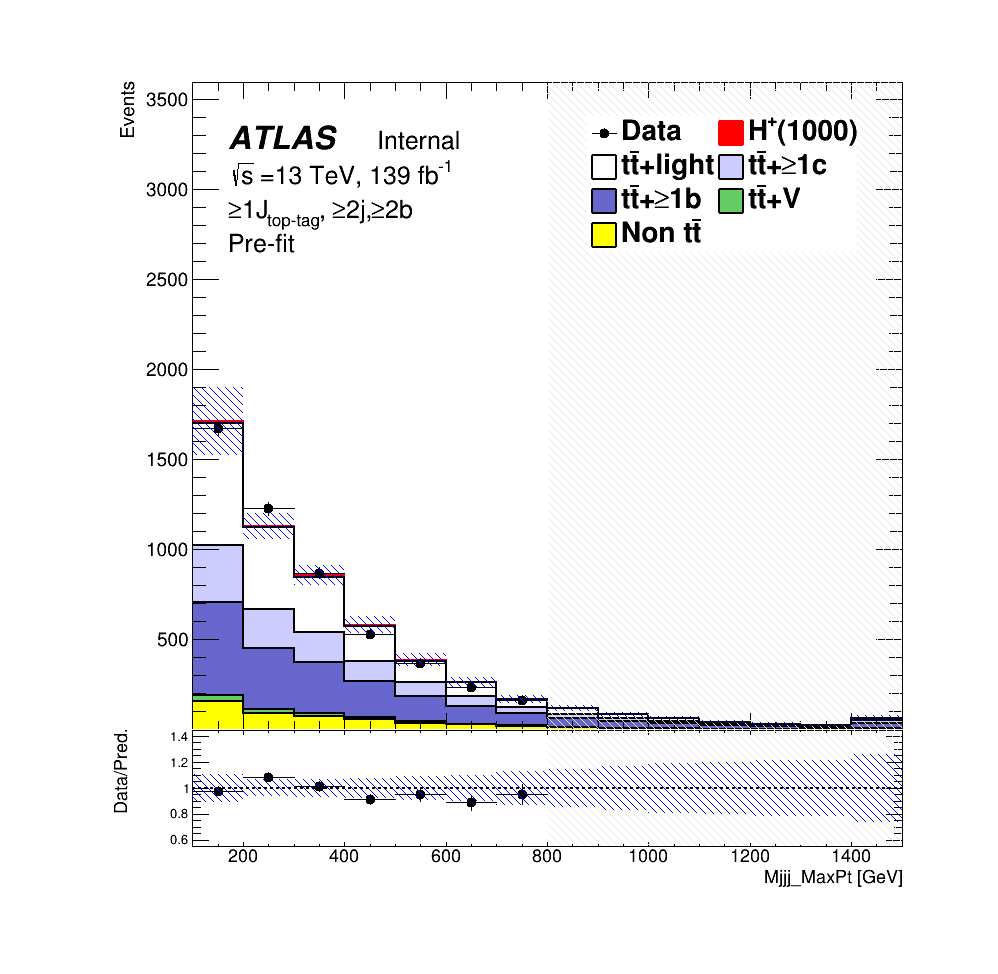
\includegraphics[width=0.50\textwidth]{images/BkgModeling/DATAOVERMC_Hp1000_Contained80_DL1r_70_Mjjj_MaxPt_beforeRW_geq1tgeq2jgeq2b_prefit.png}
        \label{fig:DATAOVERMC_Mjjj_MaxPt}
    }
\end{figure}
\begin{figure}[H]
    \addtocounter{figure}{-1}
    \subfloat[Muu\_MindR] {
        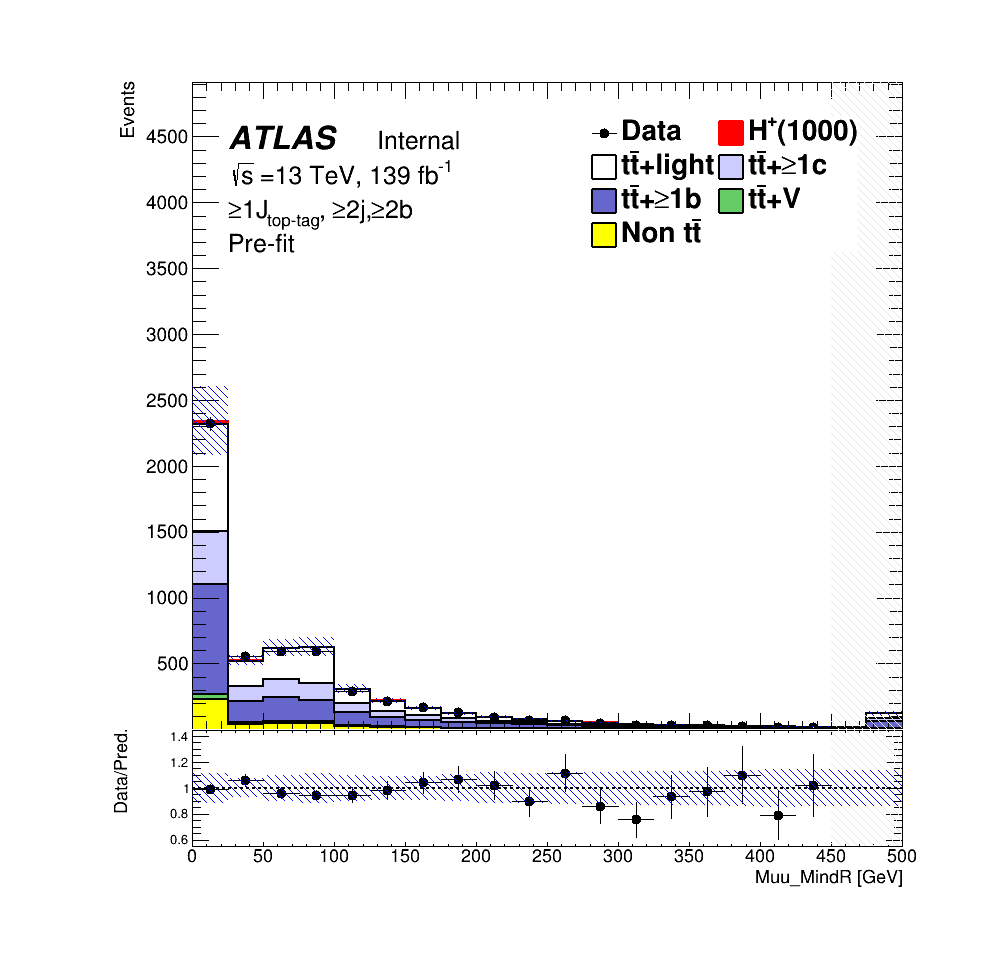
\includegraphics[width=0.50\textwidth]{images/BkgModeling/DATAOVERMC_Hp1000_Contained80_DL1r_70_Muu_MindR_beforeRW_geq1tgeq2jgeq2b_prefit.png}
        \label{fig:DATAOVERMC_Muu_MindR}
    }
    \subfloat[dRbb\_avg] {
        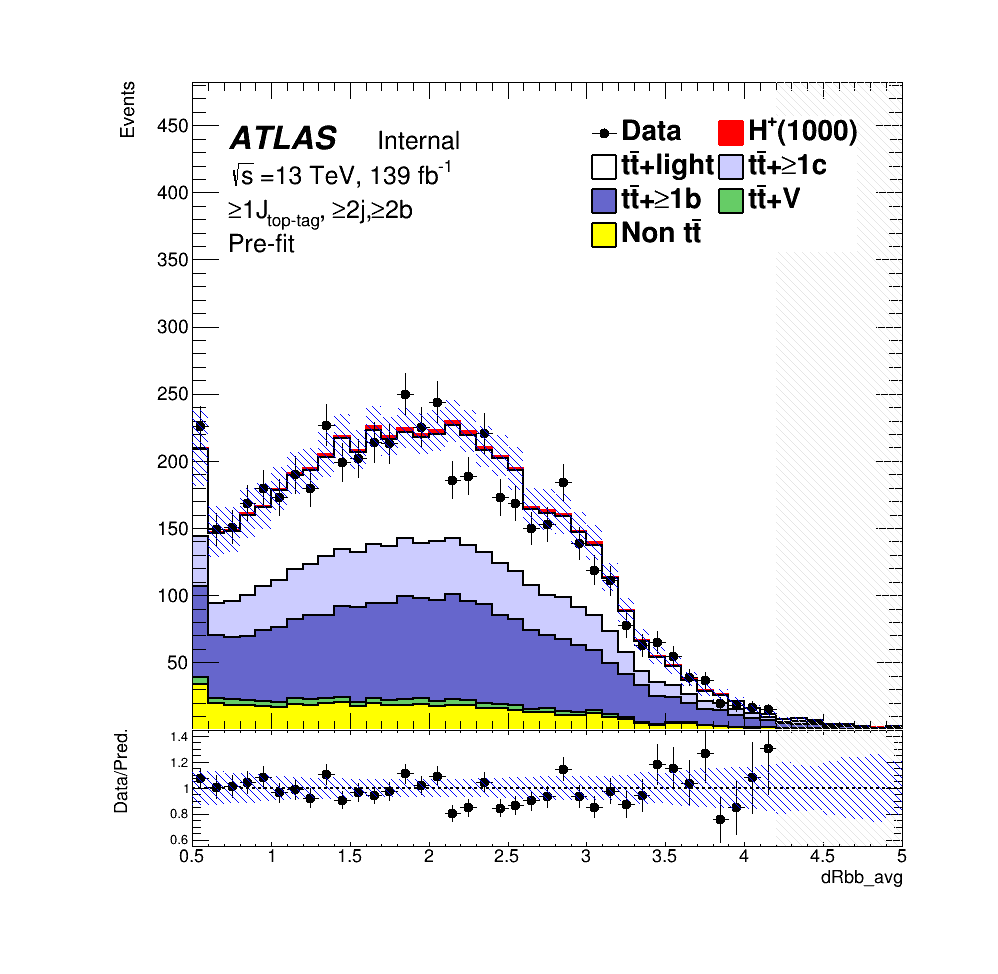
\includegraphics[width=0.50\textwidth]{images/BkgModeling/DATAOVERMC_Hp1000_Contained80_DL1r_70_dRbb_avg_beforeRW_geq1tgeq2jgeq2b_prefit.png}
        \label{fig:DATAOVERMC_dRbb_avg}
    }
\end{figure}
\begin{figure}[H]
    \addtocounter{figure}{-1}
    \subfloat[dRlepbb\_MindR] {
        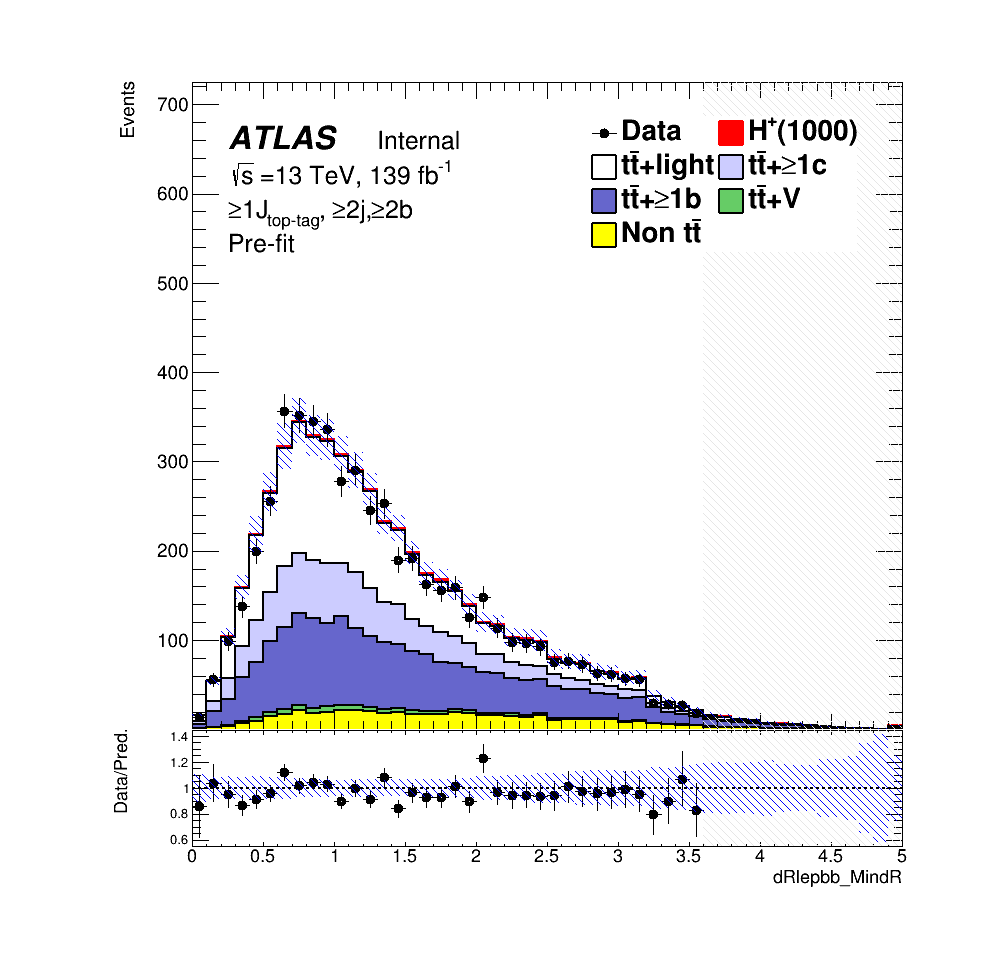
\includegraphics[width=0.50\textwidth]{images/BkgModeling/DATAOVERMC_Hp1000_Contained80_DL1r_70_dRlepbb_MindR_beforeRW_geq1tgeq2jgeq2b_prefit.png}
        \label{fig:DATAOVERMC_dRlepbb_MindR}
    }
    \subfloat[LeadingTop\_m] {
        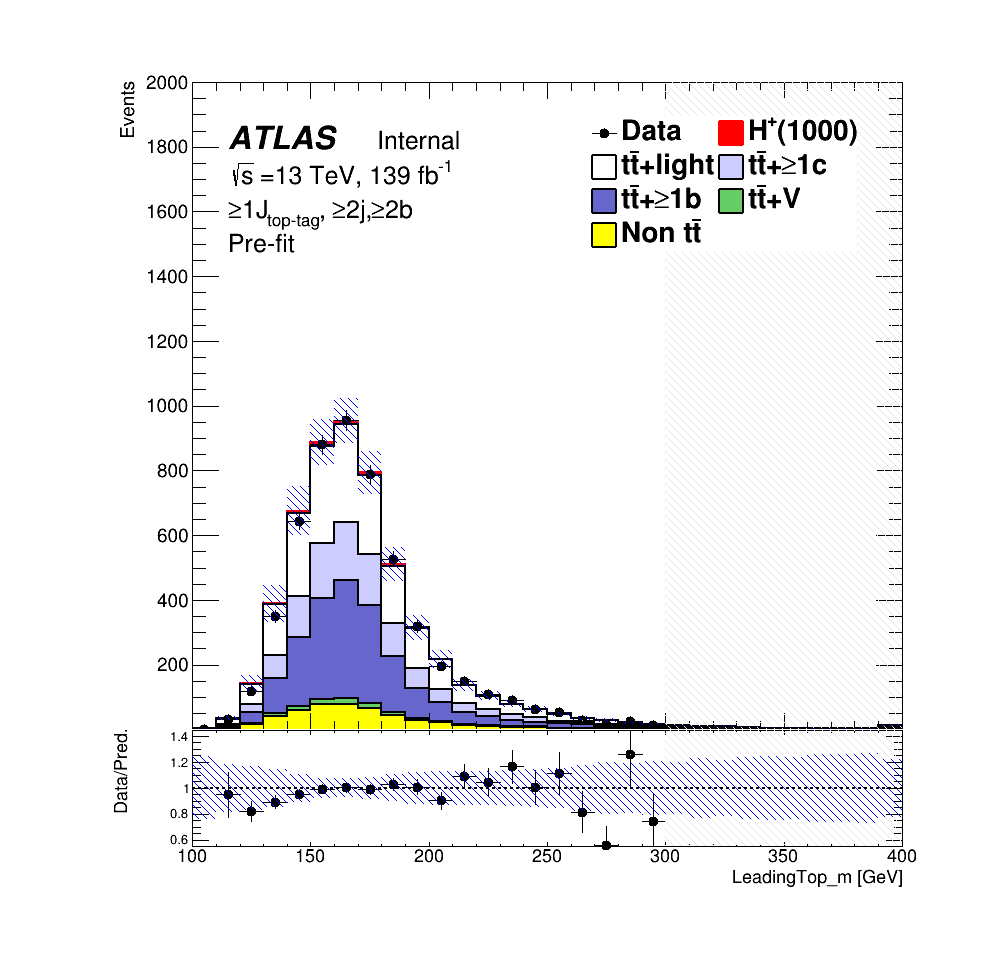
\includegraphics[width=0.50\textwidth]{images/BkgModeling/DATAOVERMC_Hp1000_Contained80_DL1r_70_LeadingTop_mass_beforeRW_geq1tgeq2jgeq2b_prefit.png}
        \label{fig:DATAOVERMC_LeadingTop_mass}
    }
\end{figure}
\begin{figure}[H]
    \addtocounter{figure}{-1}
    \subfloat[LeadingTop\_pt] {
        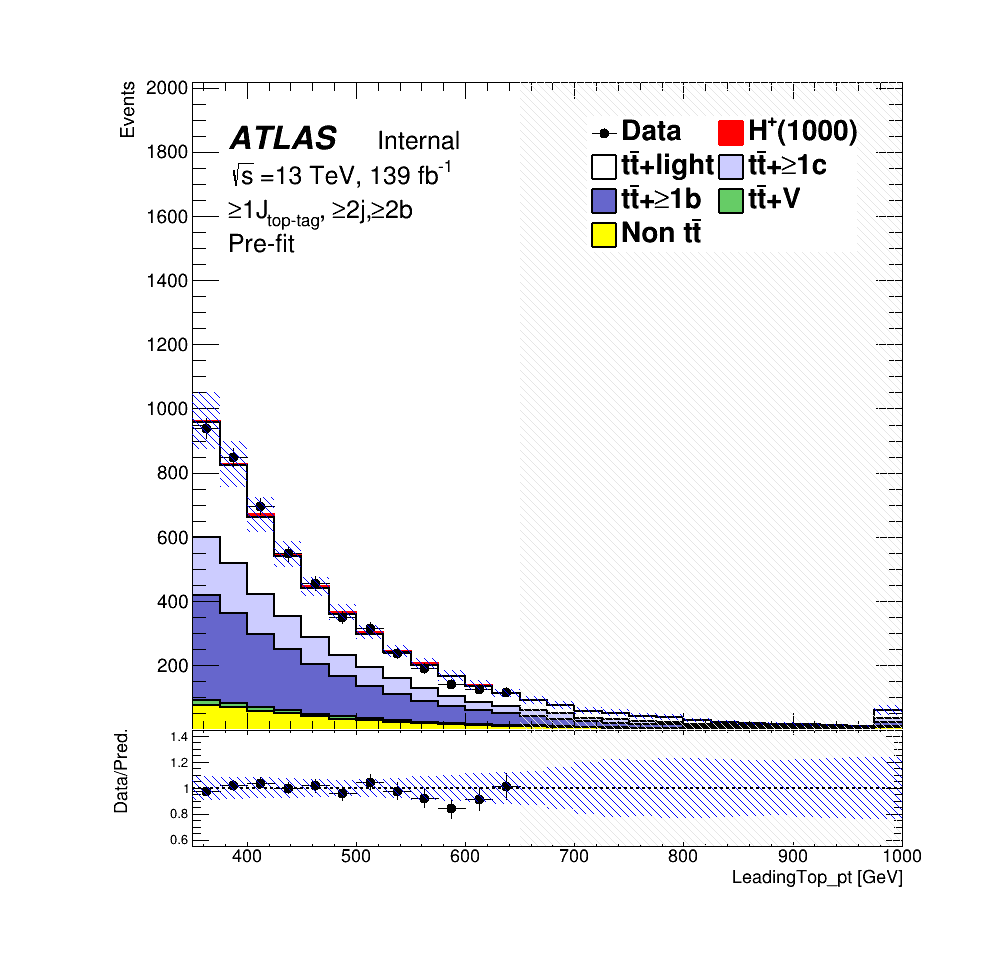
\includegraphics[width=0.50\textwidth]{images/BkgModeling/DATAOVERMC_Hp1000_Contained80_DL1r_70_LeadingTop_pt_beforeRW_geq1tgeq2jgeq2b_prefit.png}
        \label{fig:DATAOVERMC_LeadingTop_pt}
    }
    \subfloat[M\_tb] {
        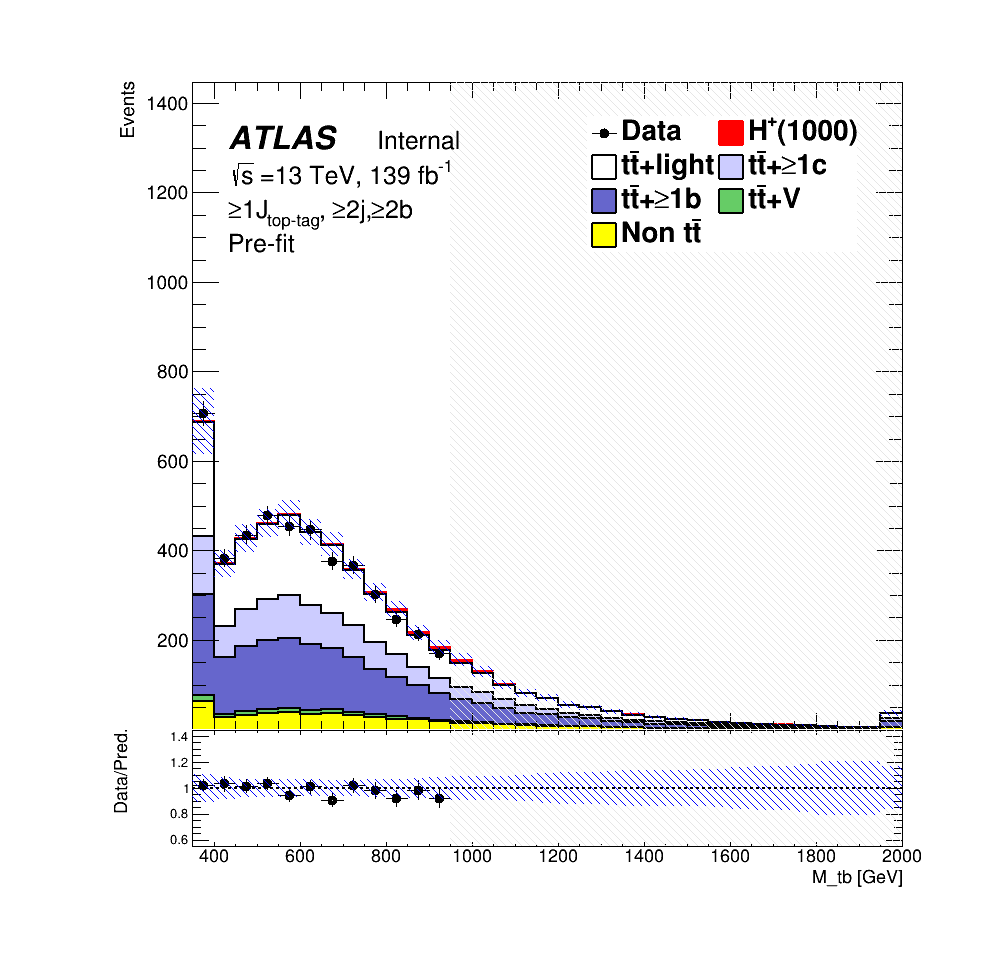
\includegraphics[width=0.50\textwidth]{images/BkgModeling/DATAOVERMC_Hp1000_Contained80_DL1r_70_tb_mass_beforeRW_geq1tgeq2jgeq2b_prefit.png}
        \label{fig:DATAOVERMC_tb_mass}
    }
\end{figure}
\begin{figure}[H]
    \addtocounter{figure}{-1}
    \subfloat[Pt\_tb] {
        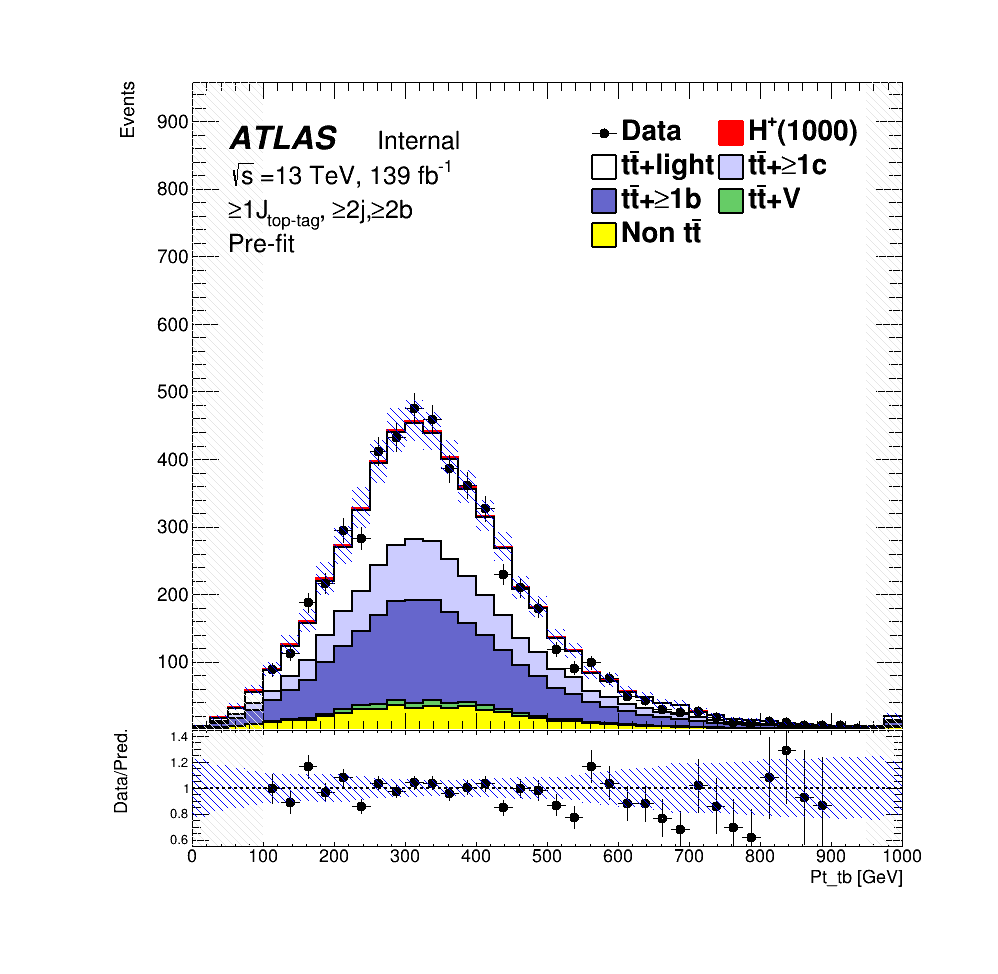
\includegraphics[width=0.50\textwidth]{images/BkgModeling/DATAOVERMC_Hp1000_Contained80_DL1r_70_tb_pt_beforeRW_geq1tgeq2jgeq2b_prefit.png}
        \label{fig:DATAOVERMC_tb_pt}
    }
    \subfloat[PtAsymm\_tb] {
        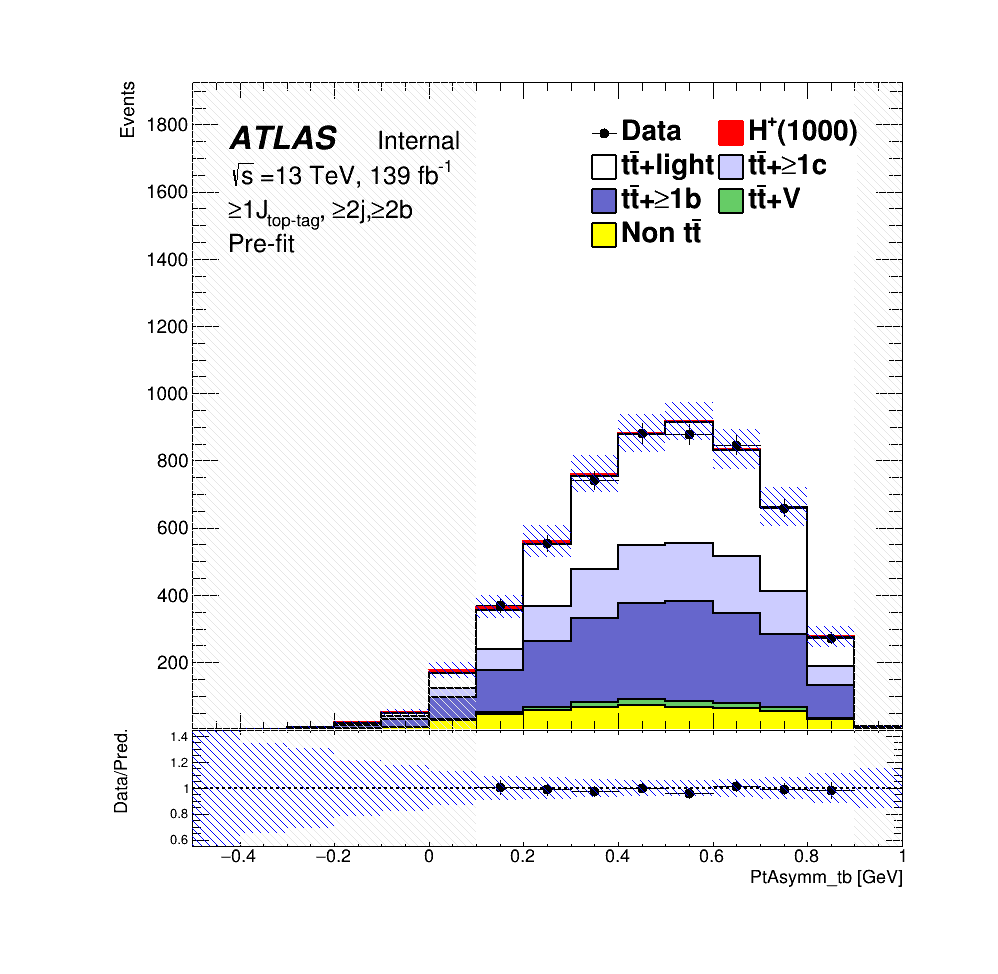
\includegraphics[width=0.50\textwidth]{images/BkgModeling/DATAOVERMC_Hp1000_Contained80_DL1r_70_tb_ptAsymm_beforeRW_geq1tgeq2jgeq2b_prefit.png}
        \label{fig:DATAOVERMC_tb_ptAsymm}
    }
  \caption{Comparison of the kinematic variables included in the BDT in the SR for the data and MC.}
  \label{fig:DATAOVERMC_BDTInputs_Prefit}
\end{figure}


\subsection{Data/MC comparison for BDT outputs}
\label{subsec:DataAndMCComparisonOfBDT}
Figures \ref{fig:DataMCComparison_BDT_Hp1000_beforeRW} to \ref{fig:DataMCComparison_BDT_Hp3000_beforeRW} show the distributions of BDT output in the SR1 and SR2. The binning of each BDT output is optimized for the search sensitivity by \textit{TransfoD} algorithm \cite{Binning-TTHFilter}. Such binning results in extremely narrow bins towards high BDT scored, and makes the plot hard to see as shown in Figure \ref{fig:SOVERB_bdt_beforeRW_geq1tgeq2jgeq2b} in Appendix \ref{subapp:SOVERB_BDTOutput} when plotted in a usual manner. We rather show the distribution with an equal interval for each bin. The distributions are input into the profile likelihood fit on each $H^{+}$ mass hypothesis as shown in Section \ref{sec:ProfileLikelohoodFit}. It is observed that the data/MC ratio tends to be lower for the high BDT score regions, which may bias the search for the signal in the highest BDT bins. The reweighting to correct for the slope is discussed in Section \ref{subsec:ReweightingTechnique}. Data in the SR2 tends to be higher as a whole. This cause should be due to the mismodeling of the $t\bar{t}+\text{jets}$ event's cross-section. Therefore, $t\bar{t}+\text{light}$ and $t\bar{t}+\text{HF}$ yields are determined by floating them in the fit.

\begin{figure}[H]
  \subfloat[] {
    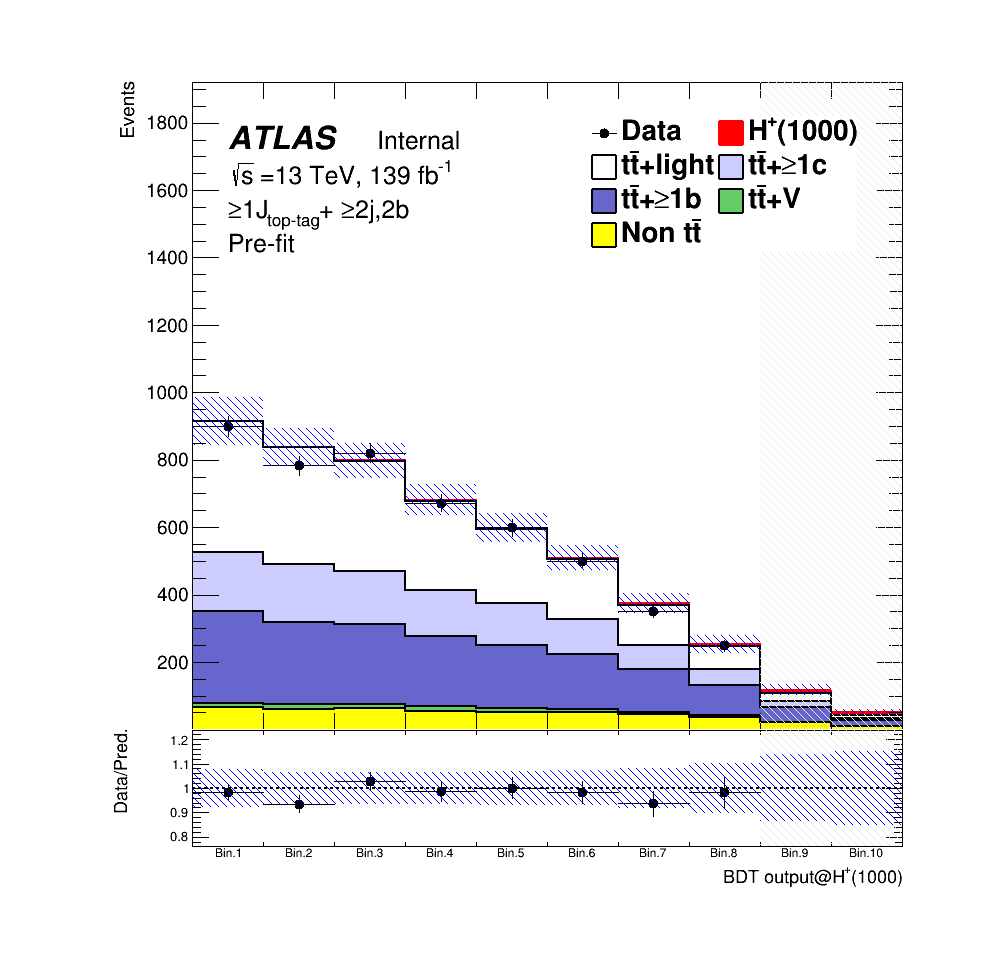
\includegraphics[width=0.50\textwidth]{images/BkgModeling/DATAOVERMC_Hp1000_Contained80_DL1r_70_bdt_Hp1000_beforeRW_geq1tgeq2j2b_prefit.png}
    \label{fig:DataMCComparison_BDT_Hp1000_SR1_beforeRW}
  }
  \subfloat[] {
    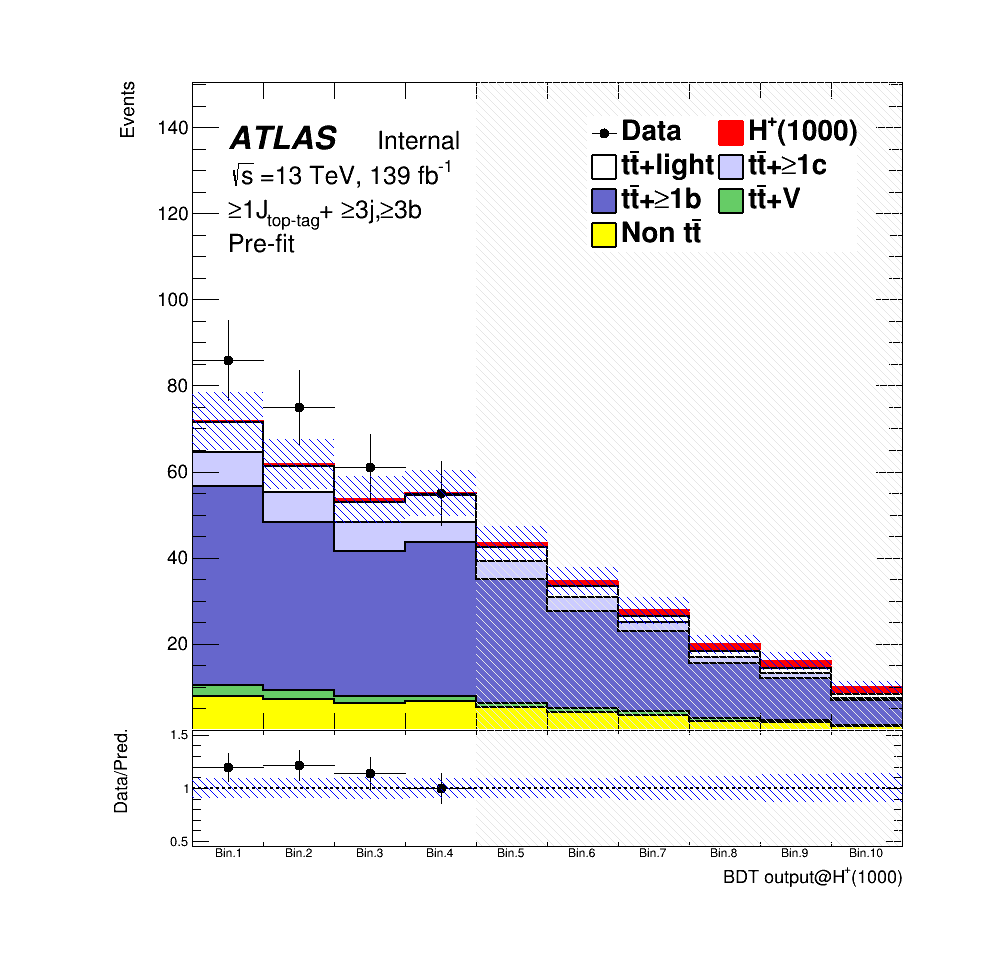
\includegraphics[width=0.50\textwidth]{images/BkgModeling/DATAOVERMC_Hp1000_Contained80_DL1r_70_bdt_Hp1000_beforeRW_geq1tgeq3jgeq3b_prefit.png}
    \label{fig:DataMCComparison_BDT_Hp1000_SR2_beforeRW}
  }
  \caption{Pre-fit distribution of BDT output trained using 1000 GeV $H^{+}$ samples in the SR1 (a) and SR2 (b).}
  \label{fig:DataMCComparison_BDT_Hp1000_beforeRW}
\end{figure}
\begin{figure}[H]
  \subfloat[] {
    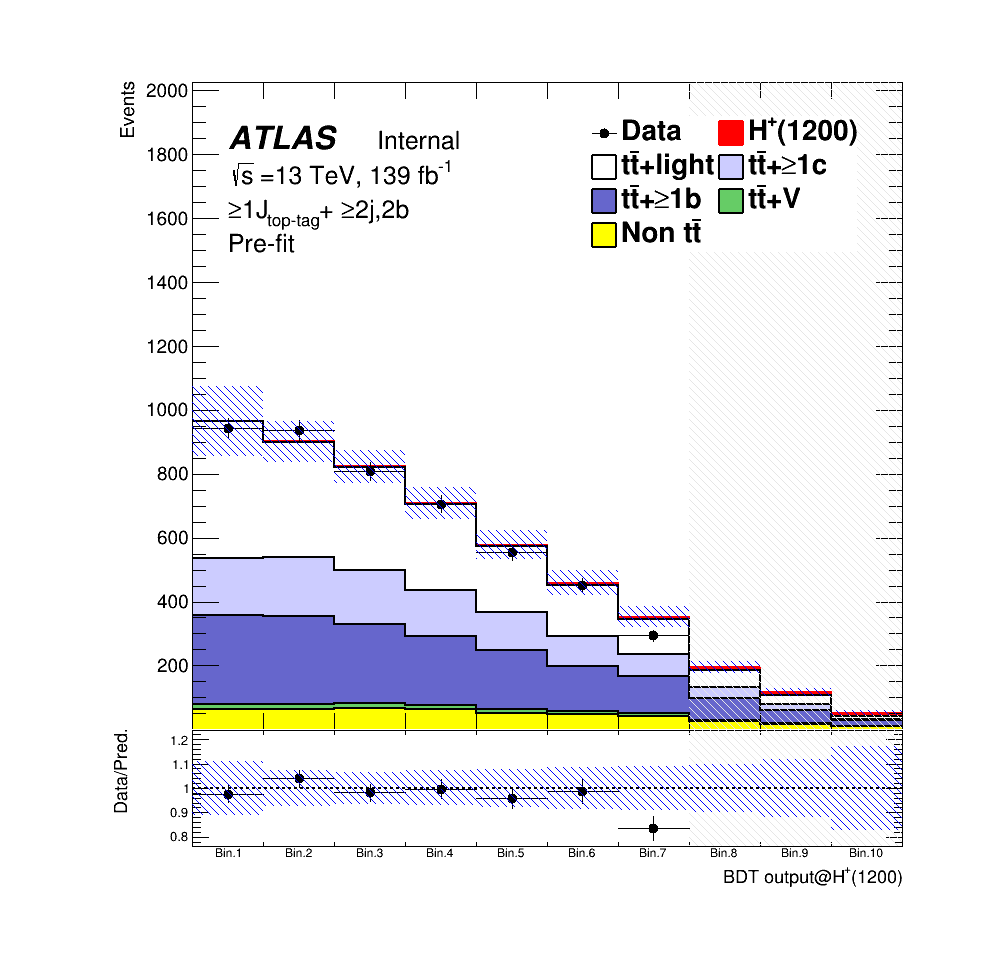
\includegraphics[width=0.50\textwidth]{images/BkgModeling/DATAOVERMC_Hp1200_Contained80_DL1r_70_bdt_Hp1200_beforeRW_geq1tgeq2j2b_prefit.png}
    \label{fig:DataMCComparison_BDT_Hp1200_SR1_beforeRW}
  }
  \subfloat[] {
    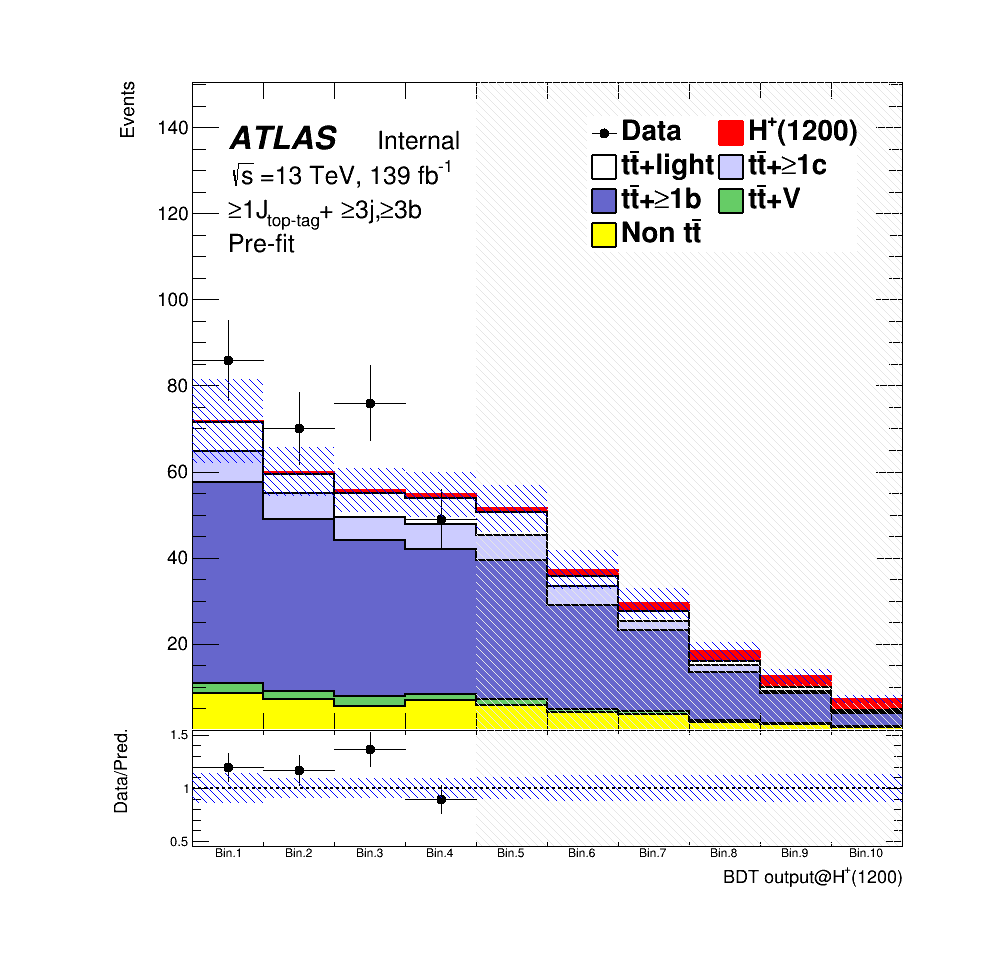
\includegraphics[width=0.50\textwidth]{images/BkgModeling/DATAOVERMC_Hp1200_Contained80_DL1r_70_bdt_Hp1200_beforeRW_geq1tgeq3jgeq3b_prefit.png}
    \label{fig:DataMCComparison_BDT_Hp1200_SR2_beforeRW}
  }
  \caption{Pre-fit distribution of BDT output trained using 1200 GeV $H^{+}$ samples in the SR1 (a) and SR2 (b).}
  \label{fig:DataMCComparison_BDT_Hp1200_beforeRW}
\end{figure}
\begin{figure}[H]
  \subfloat[] {
    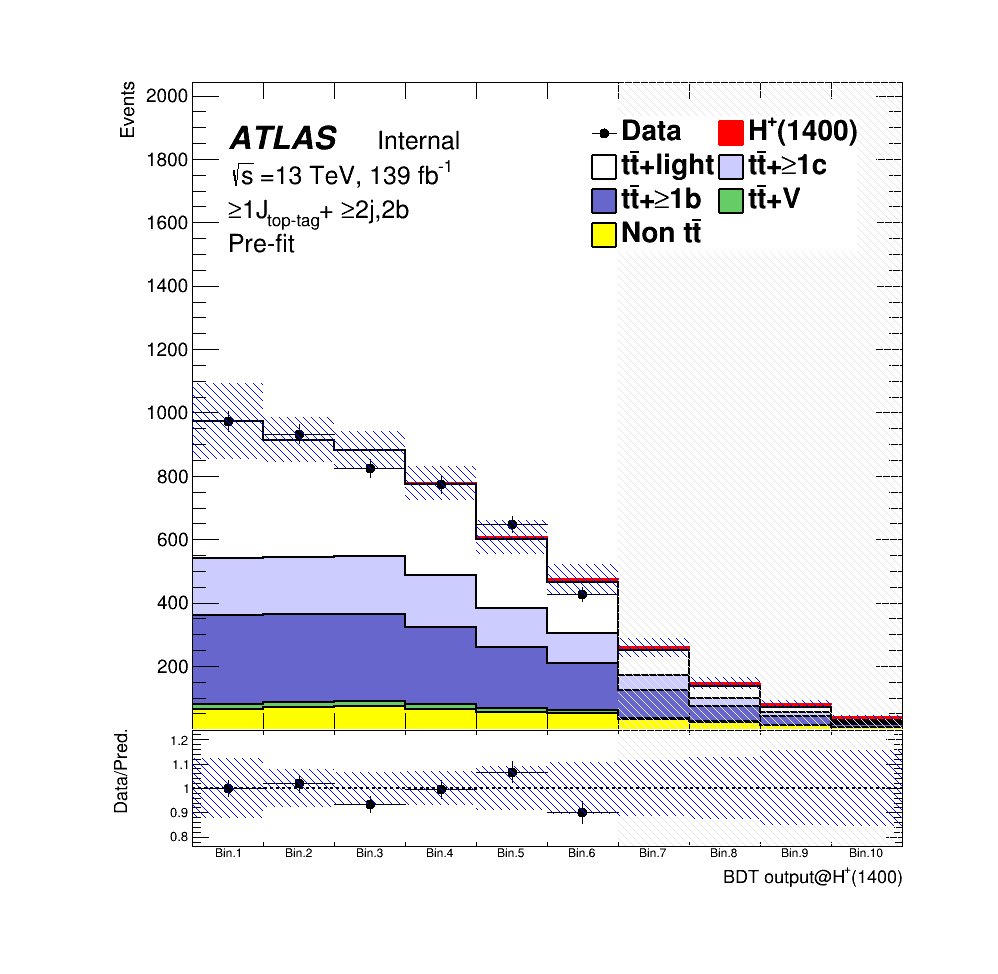
\includegraphics[width=0.50\textwidth]{images/BkgModeling/DATAOVERMC_Hp1400_Contained80_DL1r_70_bdt_Hp1400_beforeRW_geq1tgeq2j2b_prefit.png}
    \label{fig:DataMCComparison_BDT_Hp1400_SR1_beforeRW}
  }
  \subfloat[] {
    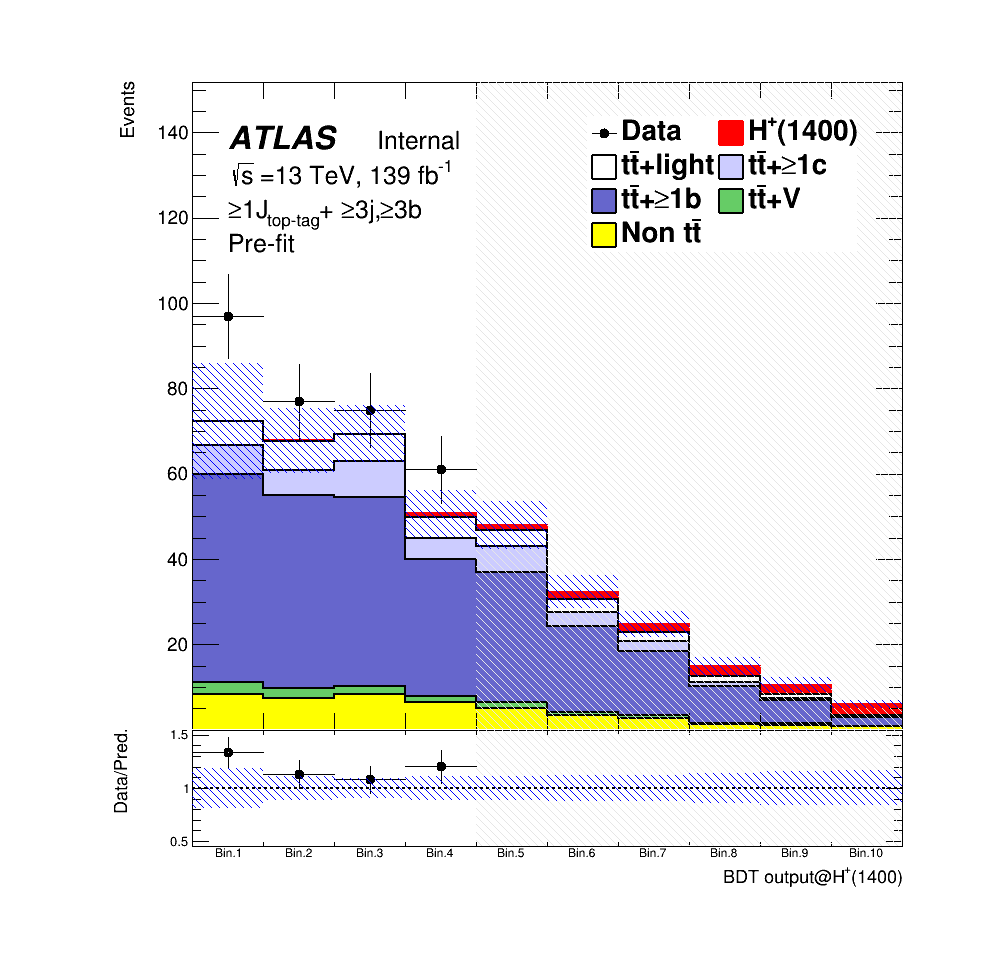
\includegraphics[width=0.50\textwidth]{images/BkgModeling/DATAOVERMC_Hp1400_Contained80_DL1r_70_bdt_Hp1400_beforeRW_geq1tgeq3jgeq3b_prefit.png}
    \label{fig:DataMCComparison_BDT_Hp1400_SR2_beforeRW}
  }
  \caption{Pre-fit distribution of BDT output trained using 1400 GeV $H^{+}$ samples in the SR1 (a) and SR2 (b).}
  \label{fig:DataMCComparison_BDT_Hp1400_beforeRW}
\end{figure}
\begin{figure}[H]
  \subfloat[] {
    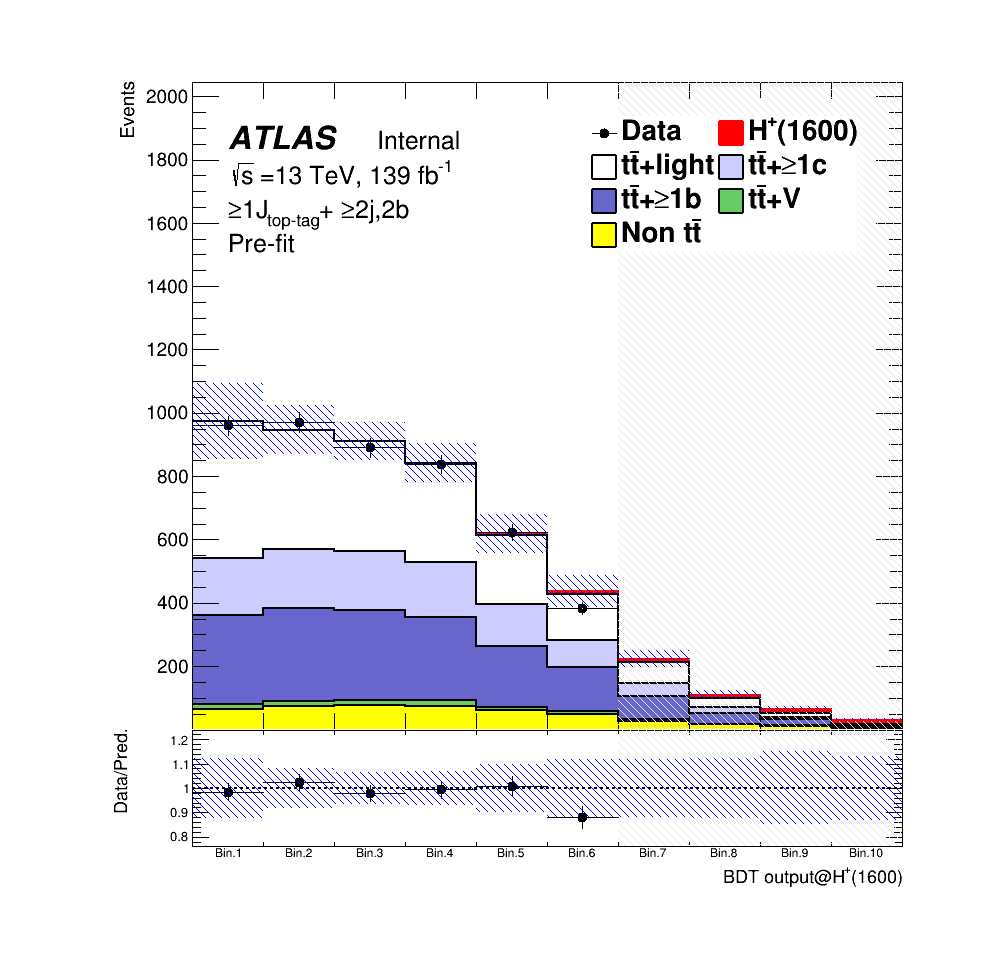
\includegraphics[width=0.50\textwidth]{images/BkgModeling/DATAOVERMC_Hp1600_Contained80_DL1r_70_bdt_Hp1600_beforeRW_geq1tgeq2j2b_prefit.png}
    \label{fig:DataMCComparison_BDT_Hp1600_SR1_beforeRW}
  }
  \subfloat[] {
    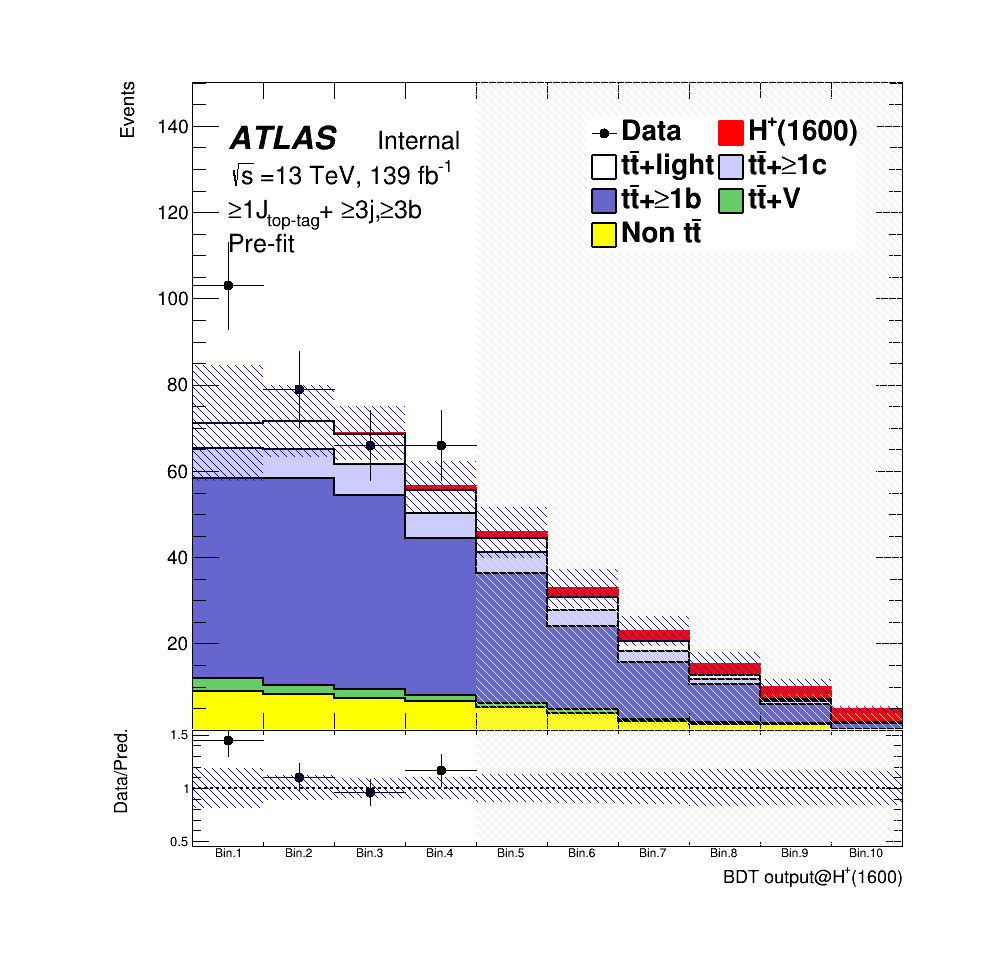
\includegraphics[width=0.50\textwidth]{images/BkgModeling/DATAOVERMC_Hp1600_Contained80_DL1r_70_bdt_Hp1600_beforeRW_geq1tgeq3jgeq3b_prefit.png}
    \label{fig:DataMCComparison_BDT_Hp1600_SR2_beforeRW}
  }
  \caption{Pre-fit distribution of BDT output trained using 1600 GeV $H^{+}$ samples in the SR1 (a) and SR2 (b).}
  \label{fig:DataMCComparison_BDT_Hp1600_beforeRW}
\end{figure}
\begin{figure}[H]
  \subfloat[] {
    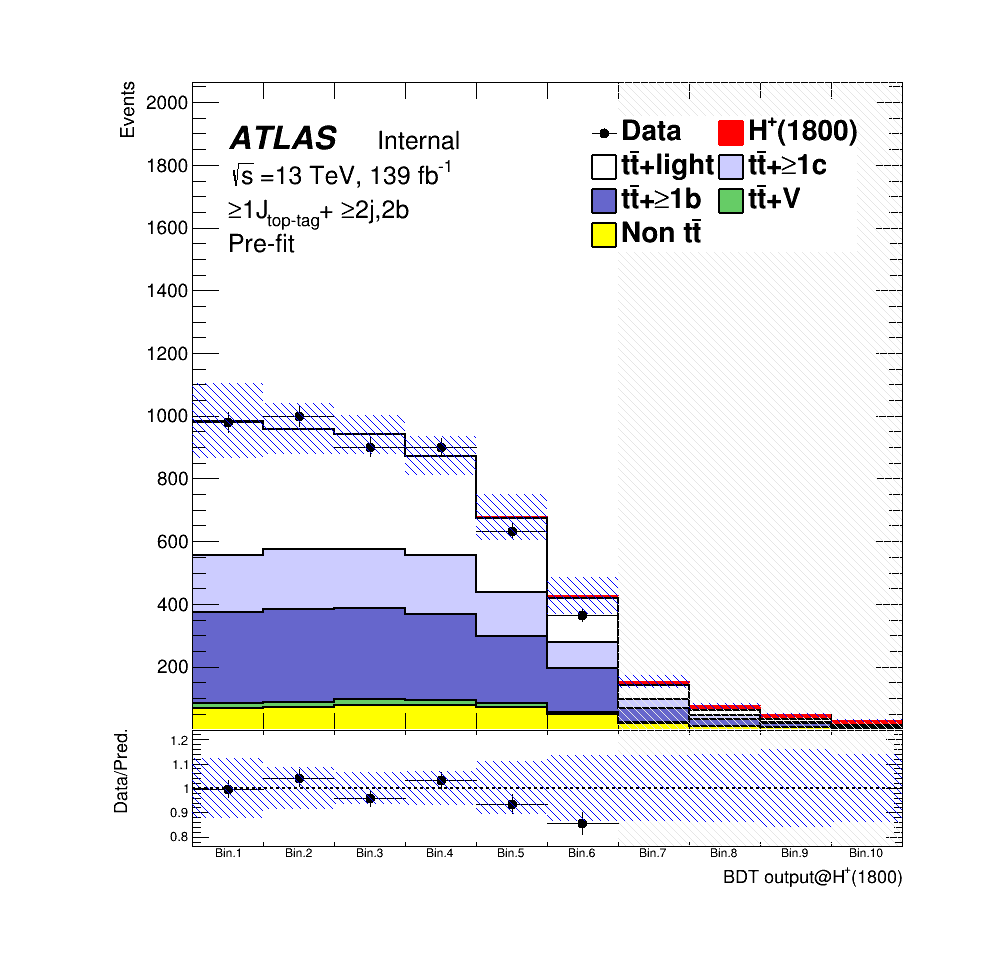
\includegraphics[width=0.50\textwidth]{images/BkgModeling/DATAOVERMC_Hp1800_Contained80_DL1r_70_bdt_Hp1800_beforeRW_geq1tgeq2j2b_prefit.png}
    \label{fig:DataMCComparison_BDT_Hp1800_SR1_beforeRW}
  }
  \subfloat[] {
    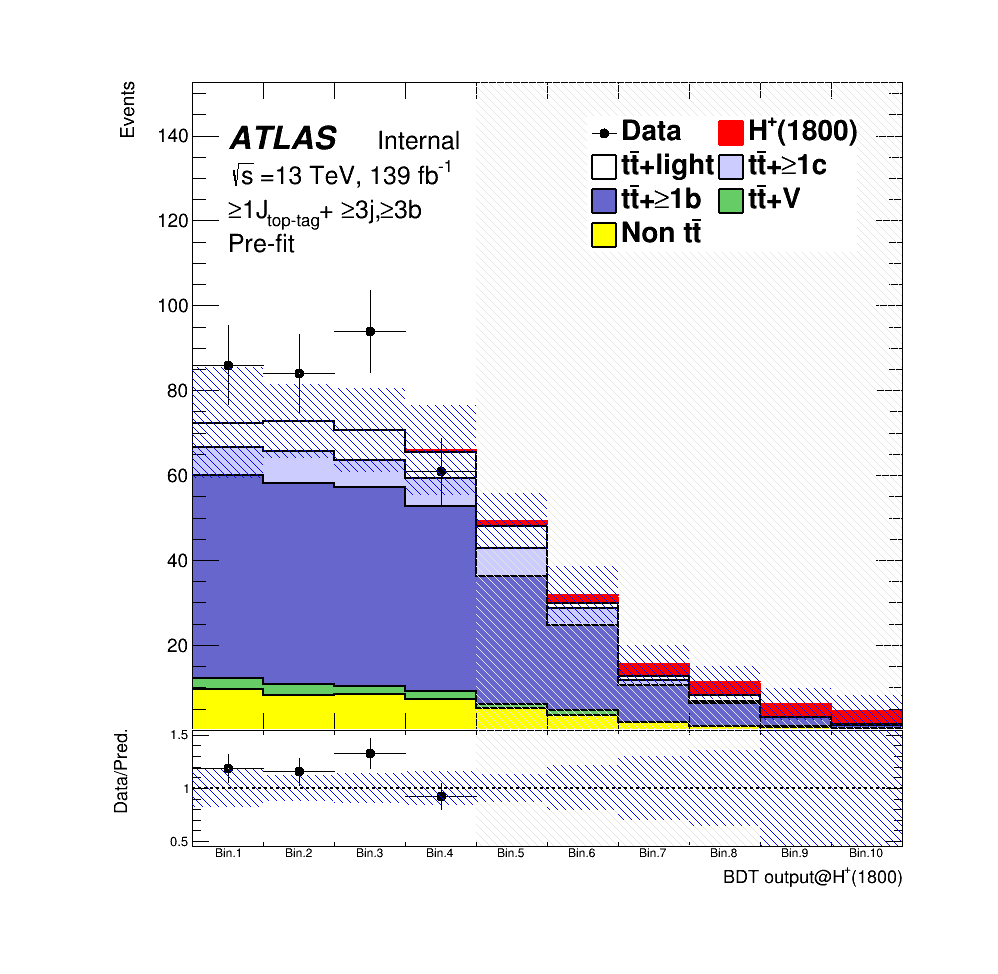
\includegraphics[width=0.50\textwidth]{images/BkgModeling/DATAOVERMC_Hp1800_Contained80_DL1r_70_bdt_Hp1800_beforeRW_geq1tgeq3jgeq3b_prefit.png}
    \label{fig:DataMCComparison_BDT_Hp1800_SR2_beforeRW}
  }
  \caption{Pre-fit distribution of BDT output trained using 1800 GeV $H^{+}$ samples in the SR1 (a) and SR2 (b).}
  \label{fig:DataMCComparison_BDT_Hp1800_beforeRW}
\end{figure}
\begin{figure}[H]
  \subfloat[] {
    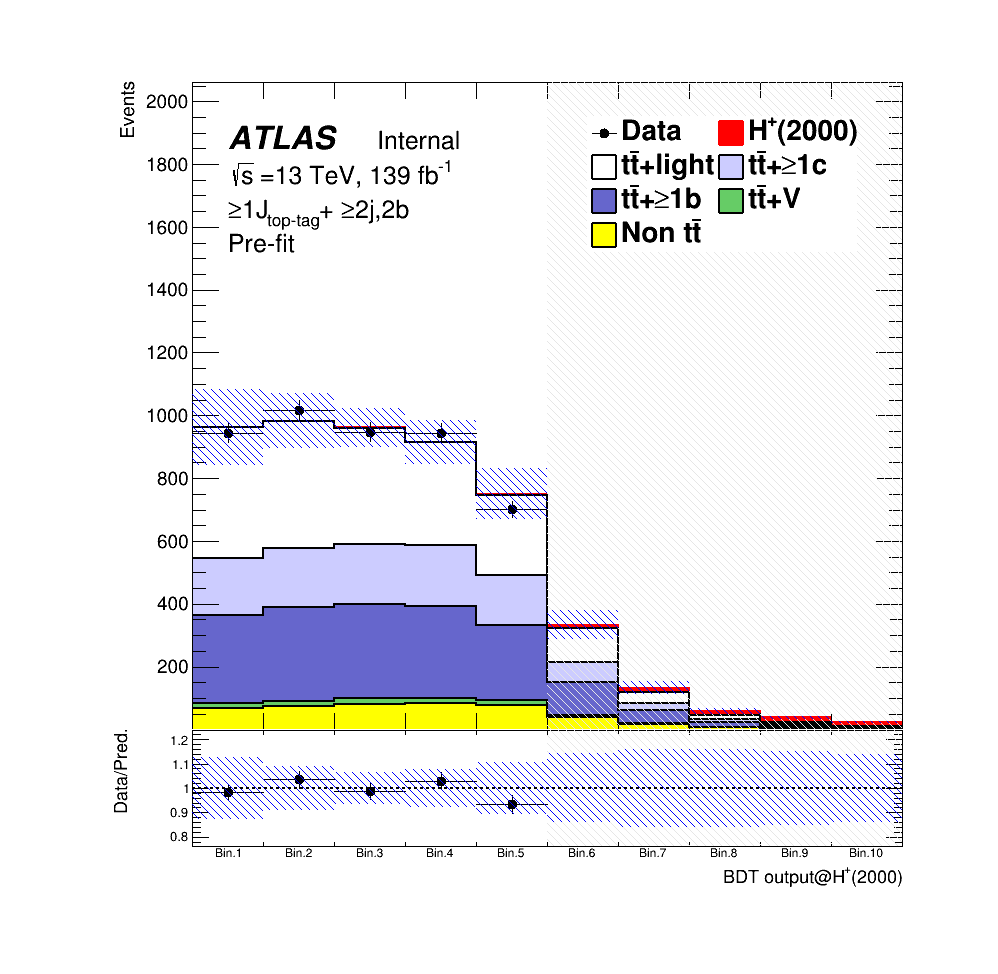
\includegraphics[width=0.50\textwidth]{images/BkgModeling/DATAOVERMC_Hp2000_Contained80_DL1r_70_bdt_Hp2000_beforeRW_geq1tgeq2j2b_prefit.png}
    \label{fig:DataMCComparison_BDT_Hp2000_SR1_beforeRW}
  }
  \subfloat[] {
    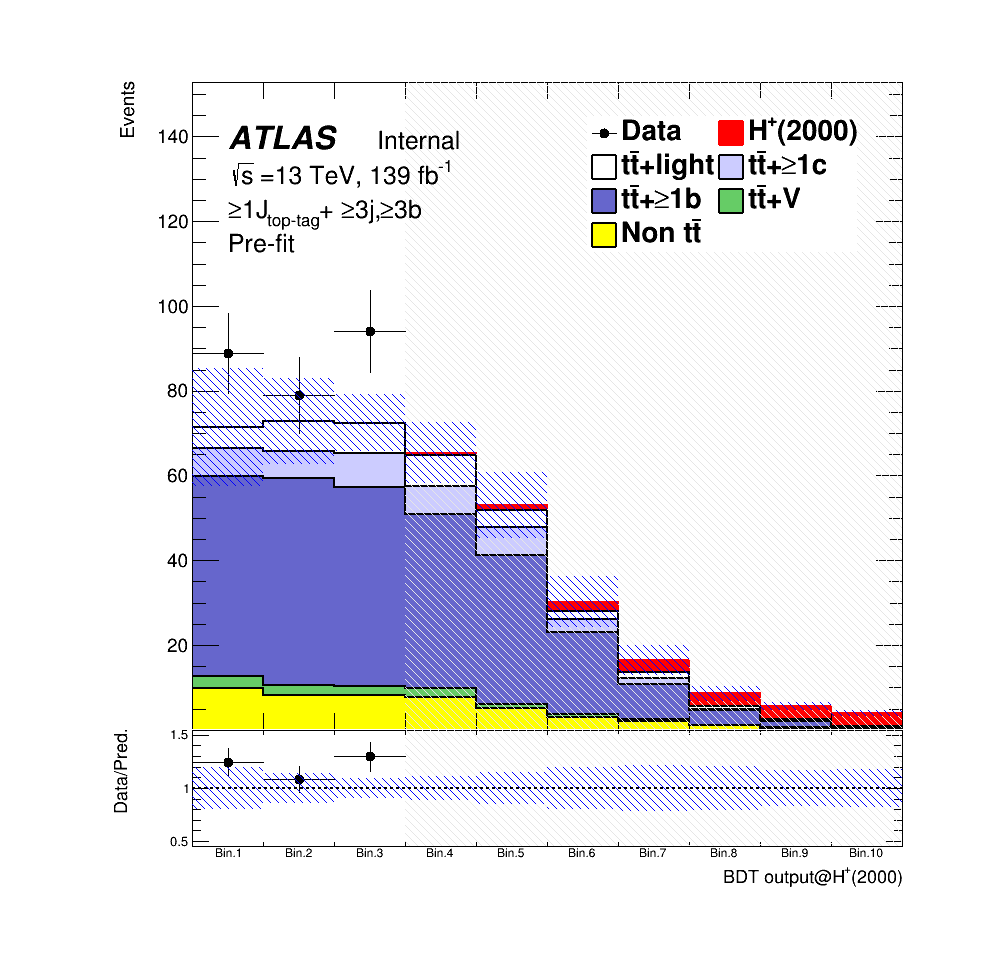
\includegraphics[width=0.50\textwidth]{images/BkgModeling/DATAOVERMC_Hp2000_Contained80_DL1r_70_bdt_Hp2000_beforeRW_geq1tgeq3jgeq3b_prefit.png}
    \label{fig:DataMCComparison_BDT_Hp2000_SR2_beforeRW}
  }
  \caption{Pre-fit distribution of BDT output trained using 2000 GeV $H^{+}$ samples in the SR1 (a) and SR2 (b).}
  \label{fig:DataMCComparison_BDT_Hp2000_beforeRW}
\end{figure}
\begin{figure}[H]
  \subfloat[] {
    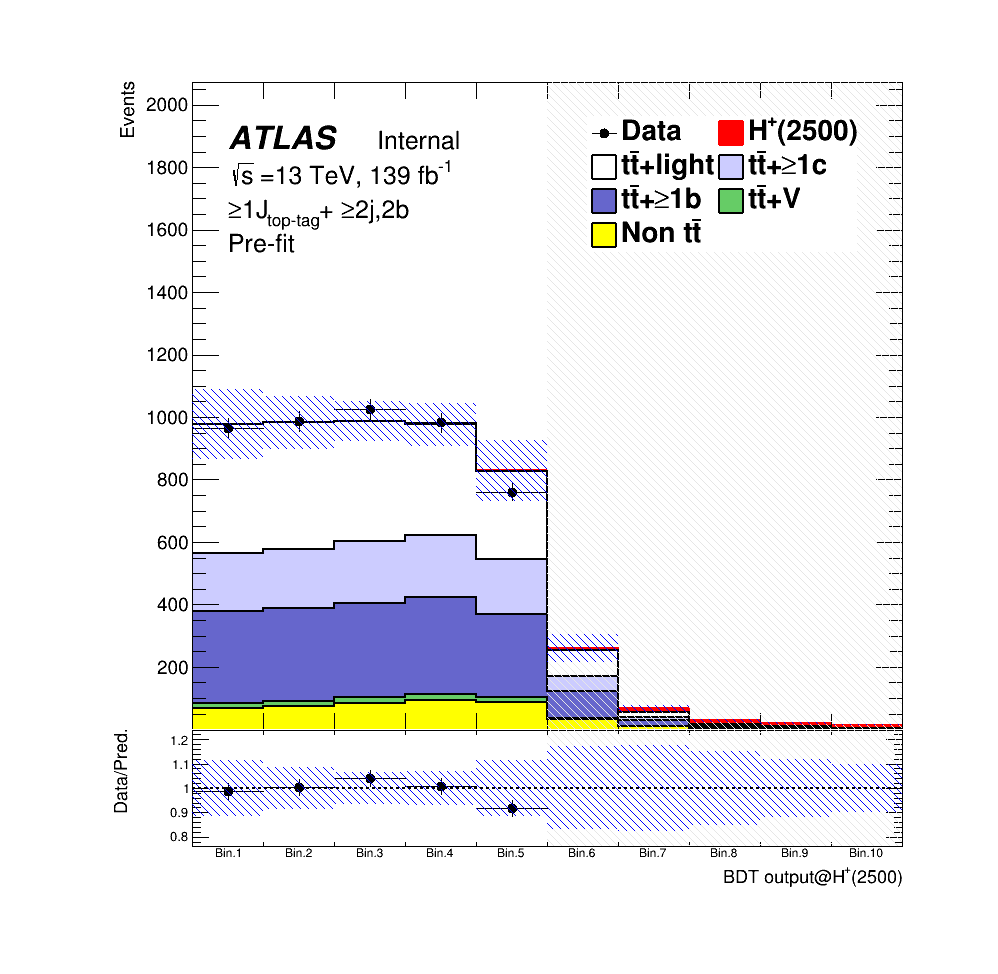
\includegraphics[width=0.50\textwidth]{images/BkgModeling/DATAOVERMC_Hp2500_Contained80_DL1r_70_bdt_Hp2500_beforeRW_geq1tgeq2j2b_prefit.png}
    \label{fig:DataMCComparison_BDT_Hp2500_SR1_beforeRW}
  }
  \subfloat[] {
    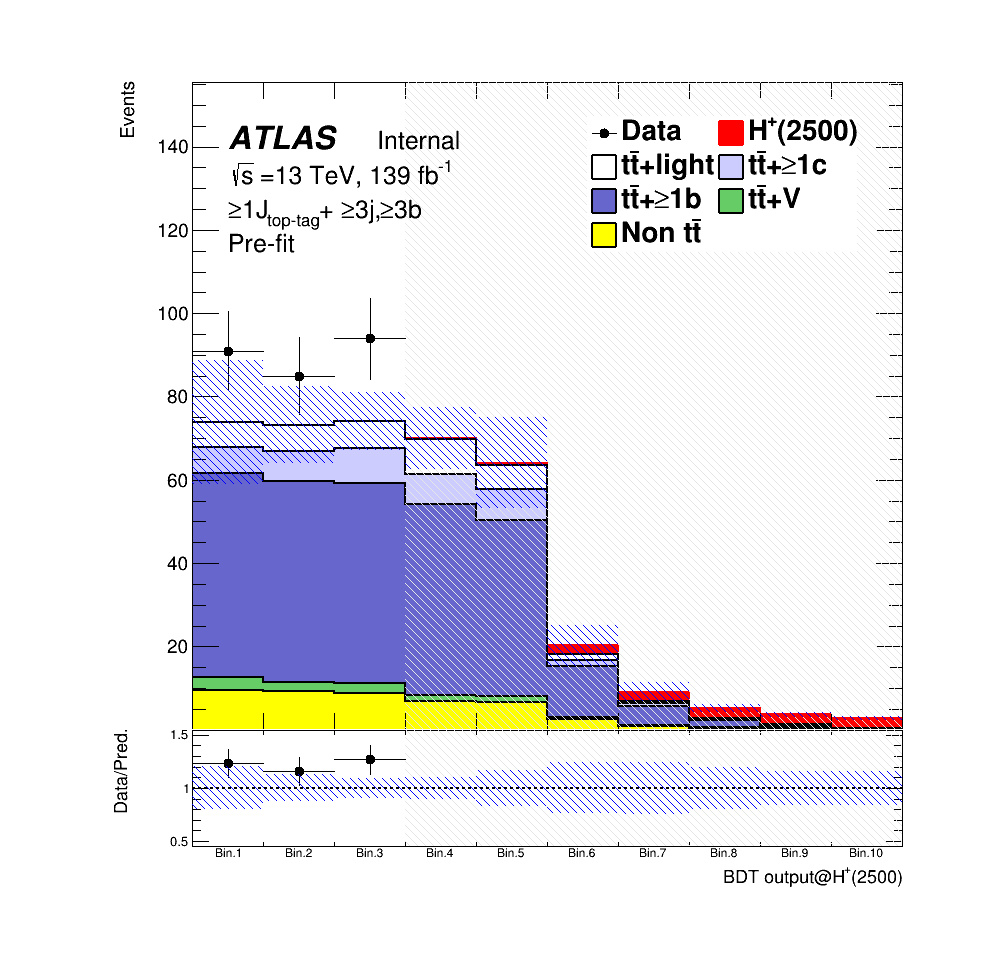
\includegraphics[width=0.50\textwidth]{images/BkgModeling/DATAOVERMC_Hp2500_Contained80_DL1r_70_bdt_Hp2500_beforeRW_geq1tgeq3jgeq3b_prefit.png}
    \label{fig:DataMCComparison_BDT_Hp2500_SR2_beforeRW}
  }
  \caption{Pre-fit distribution of BDT output trained using 2500 GeV $H^{+}$ samples in the SR1 (a) and SR2 (b).}
  \label{fig:DataMCComparison_BDT_H2500_beforeRW}
\end{figure}
\begin{figure}[H]
  \subfloat[] {
    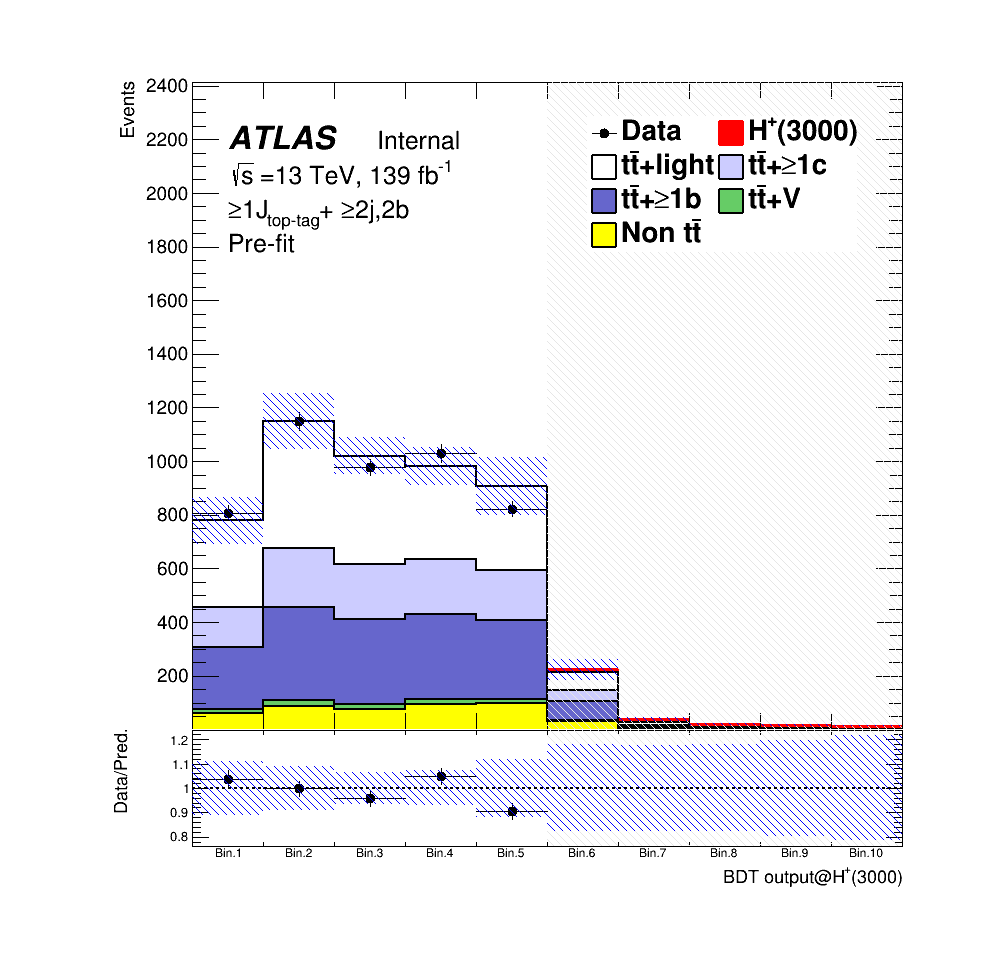
\includegraphics[width=0.50\textwidth]{images/BkgModeling/DATAOVERMC_Hp3000_Contained80_DL1r_70_bdt_Hp3000_beforeRW_geq1tgeq2j2b_prefit.png}
    \label{fig:DataMCComparison_BDT_Hp3000_SR1_beforeRW}
  }
  \subfloat[] {
    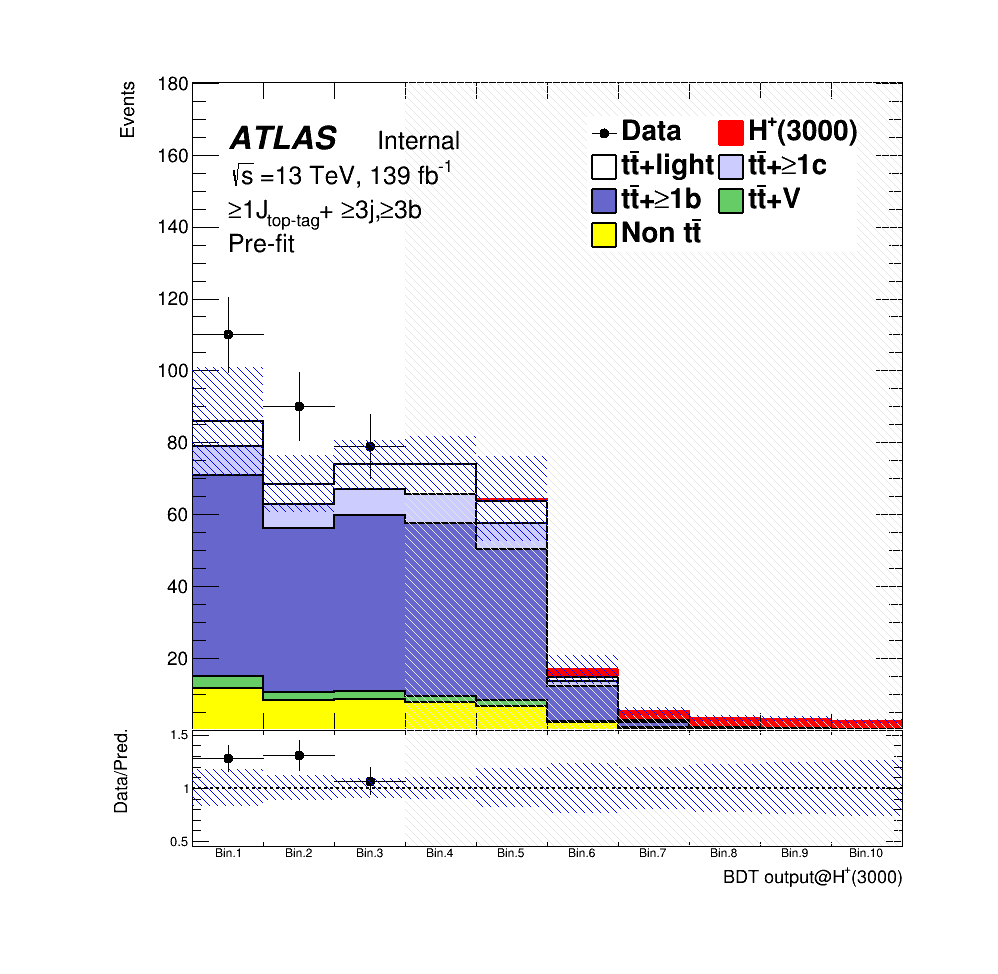
\includegraphics[width=0.50\textwidth]{images/BkgModeling/DATAOVERMC_Hp3000_Contained80_DL1r_70_bdt_Hp3000_beforeRW_geq1tgeq3jgeq3b_prefit.png}
    \label{fig:DataMCComparison_BDT_Hp3000_SR2_beforeRW}
  }
  \caption{Pre-fit distribution of BDT output trained using 3000 GeV $H^{+}$ samples in the SR1 (a) and SR2 (b).}
  \label{fig:DataMCComparison_BDT_Hp3000_beforeRW}
\end{figure}

\subsection{Reweighting technique}
\label{subsec:ReweightingTechnique}
It is known that the $t\bar{t}$ Powheg+Pythia generator does not properly model data as observed in Figure \ref{fig:DataMCComparison_BDT_Hp1000_beforeRW} to \ref{fig:DataMCComparison_BDT_Hp3000_beforeRW}. This is due to the mismodeling of the hard and soft jets. These mismodelings appear in the $p_\text{T}$ distribution of the leading top-tagged large-R jet (LeadingTop\_pt) and the invariant mass distribution of small-R jet triplet with maximum $p_{\text{T}}$ (Mjjj\_MaxPt) (these small-R jets are mainly QCD jets) as shown in Figure \ref{fig:DataMCComparison_In_LowBDTSocreRegion}, which are plotted for events in the low BDT score regions.

\begin{figure}[H]
  \subfloat[] {
    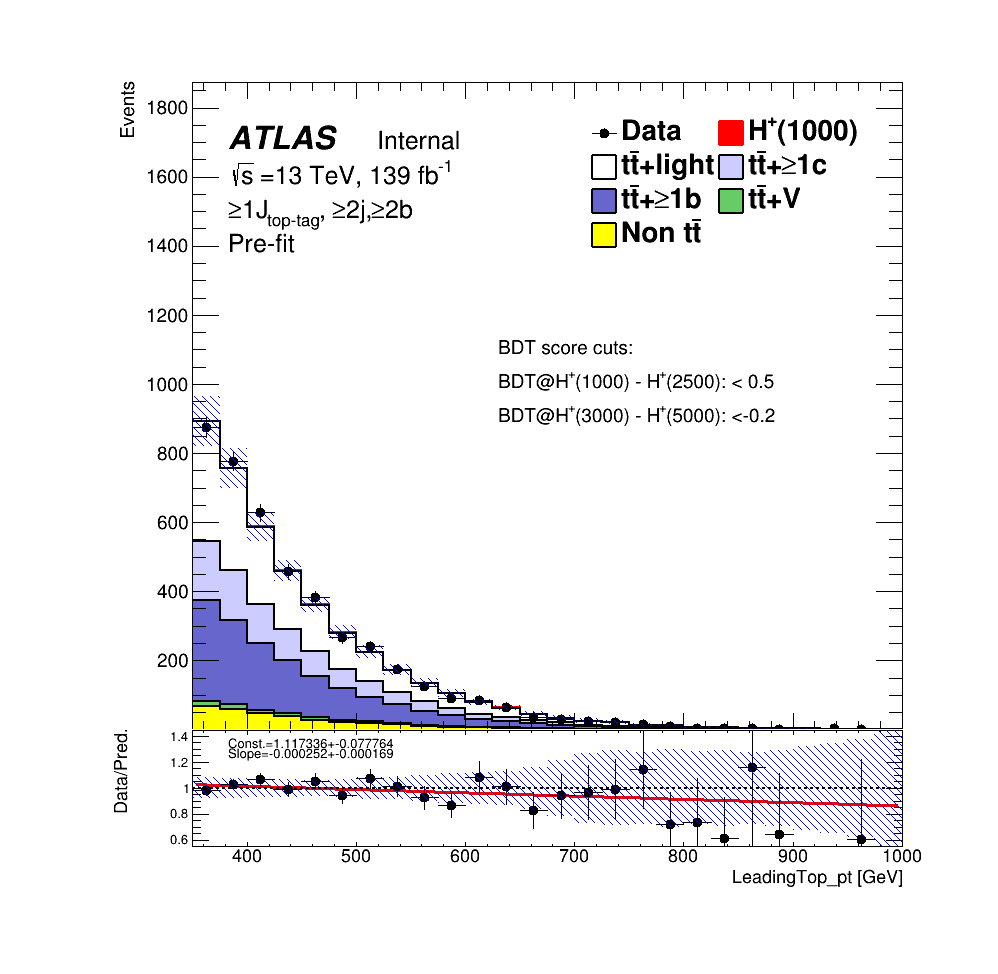
\includegraphics[width=0.50\textwidth]{images/BkgModeling/DATAOVERMC_Hp1000_Contained80_DL1r_70_LeadingTop_pt_LowBDTScore_beforeRW_geq1tgeq2jgeq2b_prefit.png}
    \label{fig:LeadingTop_pt_Modeling_LowBDTScoreEvents}
  }
  \subfloat[] {
    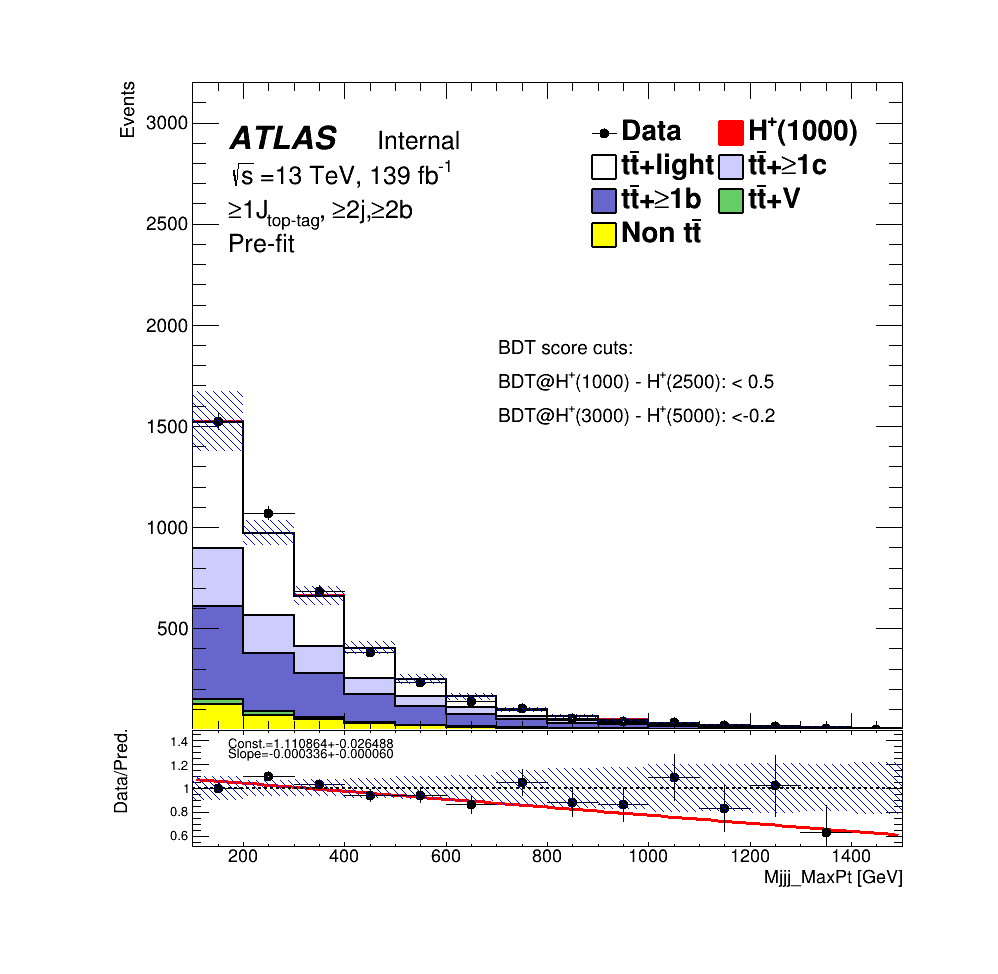
\includegraphics[width=0.50\textwidth]{images/BkgModeling/DATAOVERMC_Hp1000_Contained80_DL1r_70_Mjjj_MaxPt_LowBDTScore_beforeRW_geq1tgeq2jgeq2b_prefit.png}
    \label{fig:Mjjj_MaxPt_Modeling_LowBDTScoreEvents}
  }
  \caption{$p_{\text{T}}$ distribution of the leading top-tagged large-R jet (a) and invariant mass distribution of small-R jet triplet with maximum $p_{\text{T}}$ (b) in the low BDT score regions. Each data/MC ratio plot has a slope.}
  \label{fig:DataMCComparison_In_LowBDTSocreRegion}
\end{figure}


To improve the poor prediction of $t\bar{t}+\text{jets}$, data-based corrections are applied to the MC prediction. The reweighing factors are derived by comparing the $H_{\text{T}}^{\text{jets}}$ distribution between data and MC prediction in the inclusive SR region (i.e., SR1+SR2) because $H_{\text{T}}^{\text{jets}}$ has both hard and soft jet information. For deriving reweighting factors, events in the only low BDT score region are selected to avoid being reweighted signal events. These events are required to pass all BDT cuts under different mass hypotheses, as shown in Table \ref{tab:ReqForRWControlRegion}. Firstly, the data/MC ratios $R$ are derived according to the following definition:

\begin{equation}
  R = \frac{\text{Data}-\text{MC}^{\text{non-}t\bar{t}+\text{jets}}}{\text{MC}^{t\bar{t}+\text{jets}}}
\end{equation}

$t\bar{t}+\text{jets}$ includes the $t\bar{t}+\text{light}$, $t\bar{t}+\geq1c$ and $t\bar{t}+\geq1b$. The obtained $R$ distribution is fitted with a quadratic function ($f(H_{\text{T}}^{\text{jets}}) = a + b \cdot H_{\text{T}}^{\text{jets}} + c \cdot (H_{\text{T}}^{\text{jets}})^{2}$), and the function is used for reweighting. Figure \ref{fig:HTjets_LowBDTScoreRegion} shows the $H_{\text{T}}^{\text{jets}}$ distribution with BDT score cuts applied as indicated in Table \ref{tab:ReqForRWControlRegion}. Figure \ref{fig:HTjets_WeightFactor} shows the distribution of the weights derived from the $H_{\text{T}}^{\text{jets}}$ distribution and the obtained reweighting function. The function values are applied to $t\bar{t}+\text{light}$, $t\bar{t}+\geq1c$ and $t\bar{t}+\geq1b$. Table \ref{tab:ParameterOfReweightingFunction} includes the fitted values for all the parameters. The statistical errors of fitted parameters are included as systematic uncertainties in the final fitting. The reweighting factors in $H_{\text{T}}^{\text{jets}}>2057$ GeV region are used the value at $H_{\text{T}}^{\text{jets}}=2057$ GeV because the weight value of $-1\sigma$ become negative at the point.

\begin{table}[H]
  \centering
  \begin{tabular*}{70mm}{@{\extracolsep{\fill}}cc}
    \hline\hline
    Mass point [GeV] & BDT score cut\\
    \hline
    1000             & $< 0.5$\\
    1200             & $< 0.5$\\
    1400             & $< 0.5$\\
    1600             & $< 0.5$\\
    1800             & $< 0.5$\\
    2000             & $< 0.5$\\
    2500             & $< 0.5$\\
    3000             & $<-0.2$\\
    4000             & $<-0.2$\\
    5000             & $<-0.2$\\
    \hline\hline
  \end{tabular*}
  \caption{Events used for derivating weight factors are selected by cutting with BDT score under different mass hypotheses according to criteria in this table.}
  \label{tab:ReqForRWControlRegion}
\end{table}


\begin{figure}[H]
  \subfloat[] {
    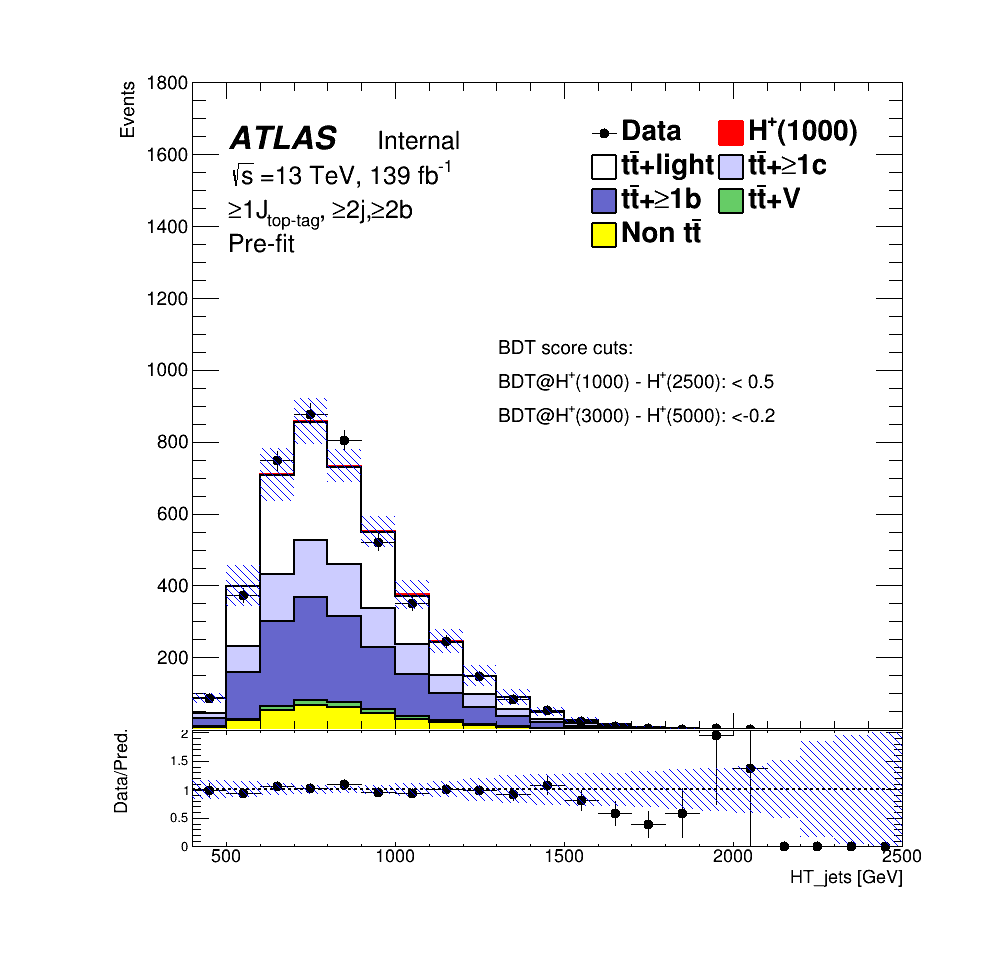
\includegraphics[width=0.50\textwidth]{images/BkgModeling/DATAOVERMC_Hp1000_Contained80_DL1r_70_HTjets_LowBDTScore_beforeRW_geq1tgeq2jgeq2b_prefit.png}
    \label{fig:HTjets_LowBDTScoreRegion}
  }
  \subfloat[] {
    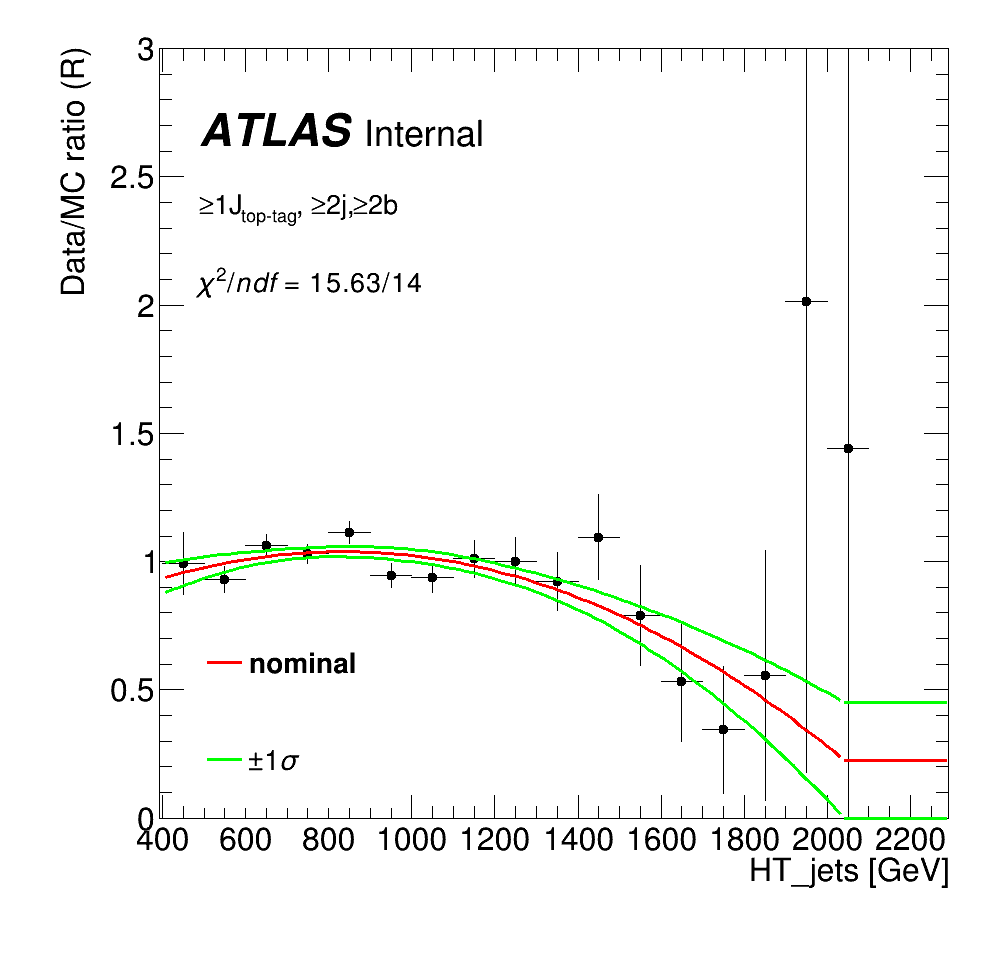
\includegraphics[width=0.48\textwidth]{images/BkgModeling/RWFunc_Hp1000_Contained80_DL1r_70_HTjets_LowBDTScore_beforeRW_geq1tgeq2jgeq2b_nominal.png}
    \label{fig:HTjets_WeightFactor}
  }
  \caption{$H_{\text{T}}^{\text{jets}}$ distribution with BDT score cuts applied (left) and the data/MC ratio distribution derived from the $H_{\text{T}}^{\text{jets}}$ distribution (right). The red function in Figure (b) is the reweighting function obtained by fitting to $R$ distribution with a quadratic function. The green ones are the stat. uncertainty (${\pm}1{\sigma}$) of the red function. They are included as systematic uncertainties in the final fitting. The reweighting factors in $H_{\text{T}}^{\text{jets}}>2057$ GeV region are assigned the value at $H_{\text{T}}^{\text{jets}}=2057$ GeV because the weight value of $-1\sigma$ become negative at the point. }
  \label{fig:HTjets_for_RW}
\end{figure}


\begin{table}[H]
  \centering
  \begin{tabular*}{60mm}{c|c}
    \hline\hline
    Parameter & Value\\
    \hline
    $a$ & $( 6.51{\pm}1.85)\times10^{-1}$ \\
    \hline
    $b$ & $( 9.30{\pm}3.93)\times10^{-4}$ \\
    \hline
    $c$ & $(-5.58{\pm}1.99)\times10^{-7}$ \\
    \hline\hline
  \end{tabular*}
  \caption{Summary of parameters obtained by fitting to the weight distribution with a quadratic function ($f(H_{\text{T}}^{\text{jets}}) = a + b \cdot H_{\text{T}}^{\text{jets}} + c \cdot (H_{\text{T}}^{\text{jets}})^{2}$). The error of each parameter is from stat. uncertainty.}
  \label{tab:ParameterOfReweightingFunction}
\end{table}


Figure \ref{fig:DataMCComparison_bdt_Hp1000_AfterRW} to Figure \ref{fig:DataMCComparison_bdt_Hp3000_AfterRW} show BDT output distributions applied to reweighting in the SR1 and SR2 region. The data/MC disagreements in the high BDT score regions have improved.

\begin{figure}[H]
  \subfloat[] {
    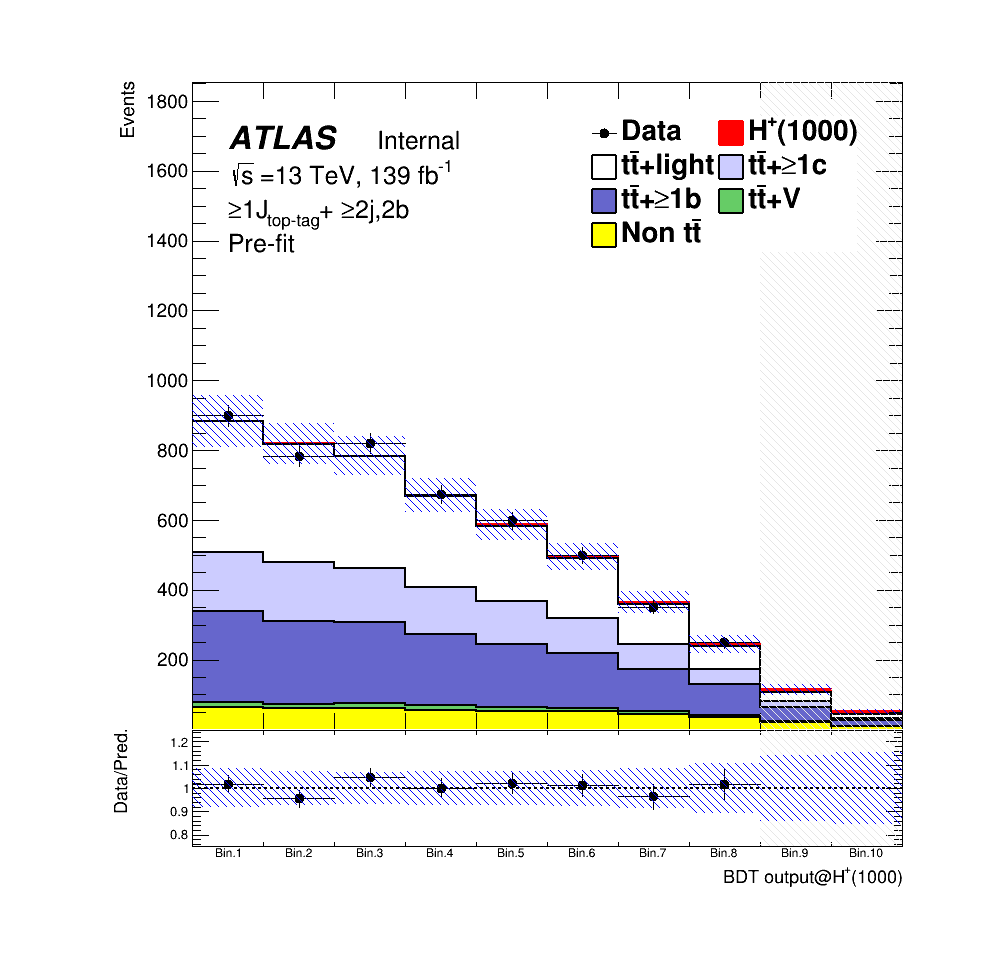
\includegraphics[width=0.50\textwidth]{images/BkgModeling/DATAOVERMC_Hp1000_Contained80_DL1r_70_bdt_Hp1000_geq1tgeq2j2b_prefit.png}
    \label{fig:BDT_Hp1000_InSR1_AfterRW}
  }
  \subfloat[] {
    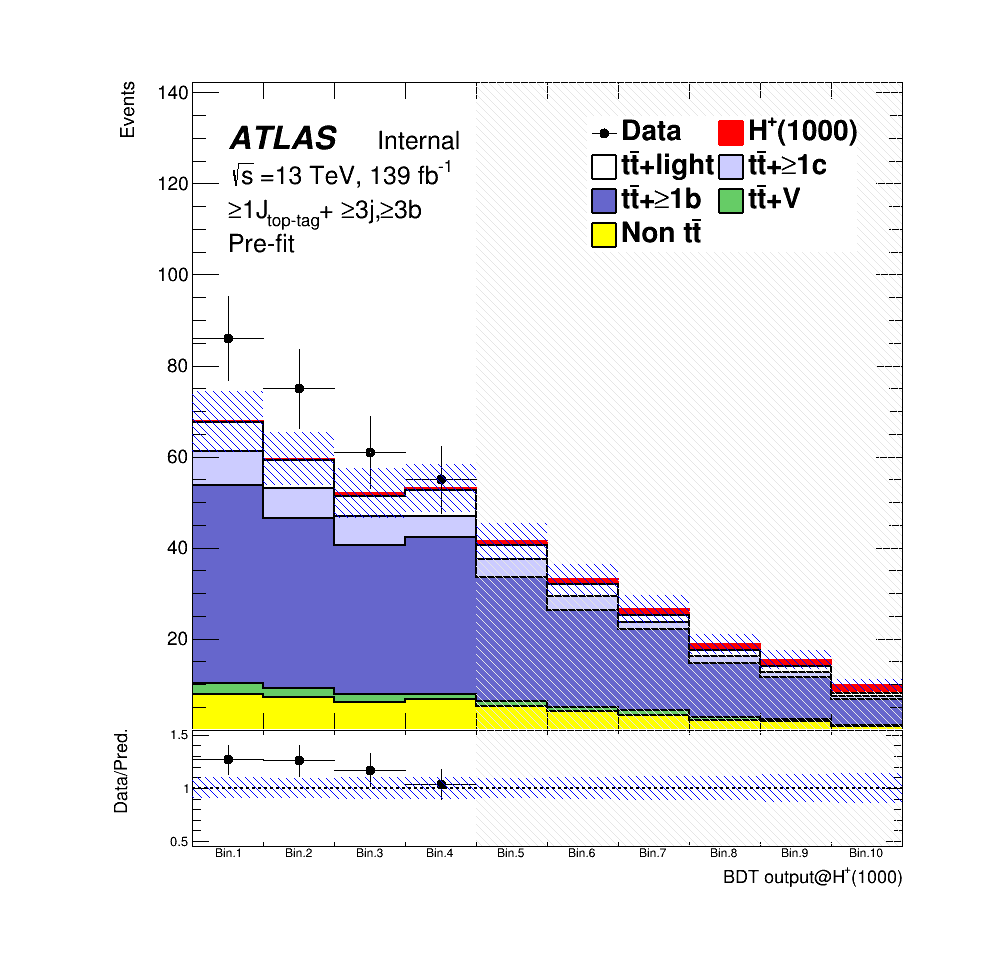
\includegraphics[width=0.50\textwidth]{images/BkgModeling/DATAOVERMC_Hp1000_Contained80_DL1r_70_bdt_Hp1000_geq1tgeq3jgeq3b_prefit.png}
    \label{fig:BDT_Hp1000_InSR2_AfterR}
  }
  \caption{Pre-fit distributions of BDT output trained using 1000 GeV $H^{+}$ in the SR1 (a) and SR2 (b) after reweighting.}
  \label{fig:DataMCComparison_bdt_Hp1000_AfterRW}
\end{figure}
\begin{figure}[H]
  \subfloat[] {
    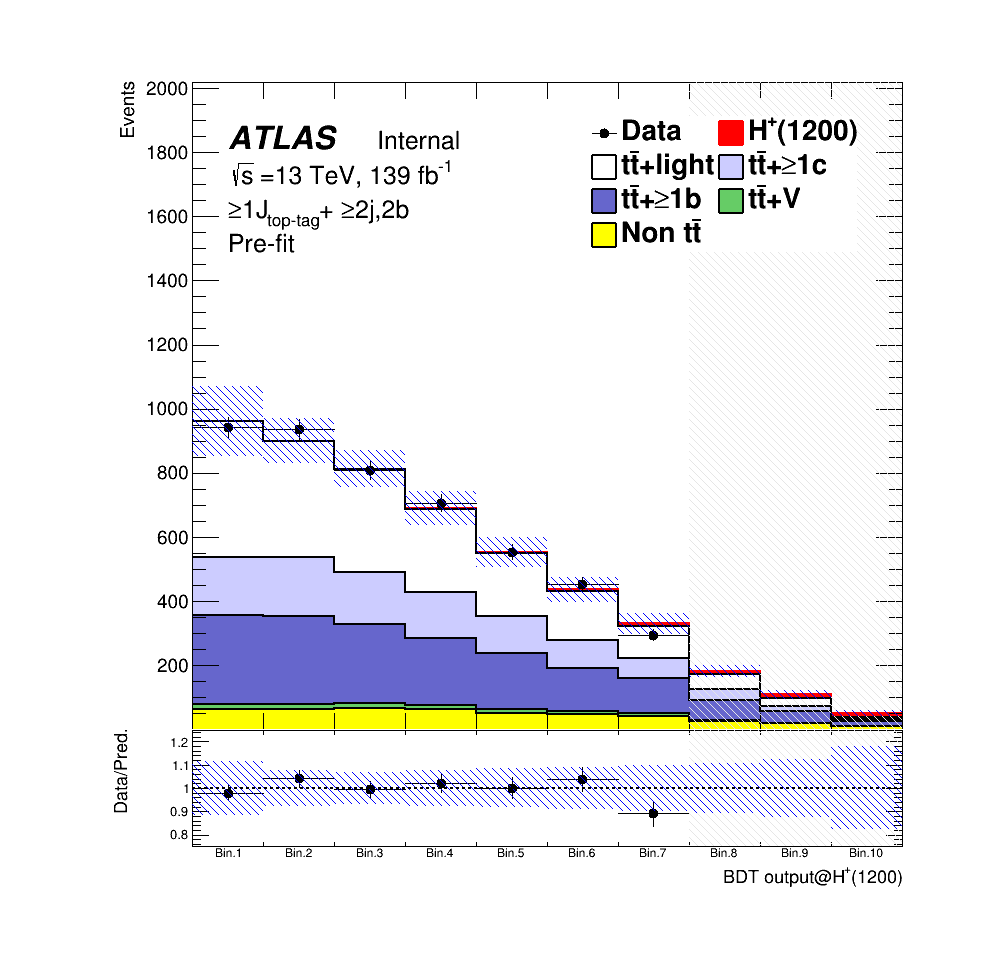
\includegraphics[width=0.50\textwidth]{images/BkgModeling/DATAOVERMC_Hp1200_Contained80_DL1r_70_bdt_Hp1200_geq1tgeq2j2b_prefit.png}
    \label{fig:BDT_Hp1200_InSR1_AfterRW}
  }
  \subfloat[] {
    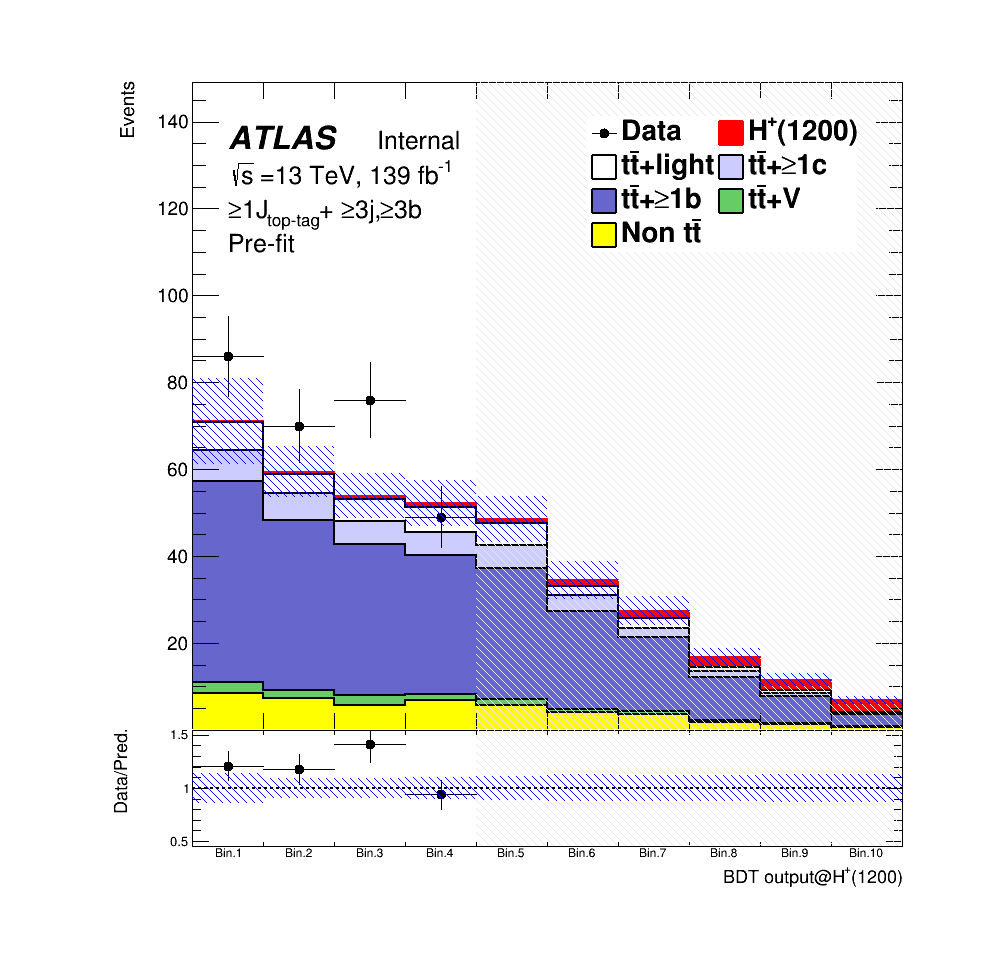
\includegraphics[width=0.50\textwidth]{images/BkgModeling/DATAOVERMC_Hp1200_Contained80_DL1r_70_bdt_Hp1200_geq1tgeq3jgeq3b_prefit.png}
    \label{fig:BDT_Hp1200_InSR2_AfterRW}
  }
  \caption{Pre-fit distributions of BDT output trained using 1200 GeV $H^{+}$ in the SR1 (a) and SR2 (b) after reweighting.}
  \label{fig:DataMCComparison_bdt_Hp1200_AfterRW}
\end{figure}
\begin{figure}[H]
  \subfloat[] {
    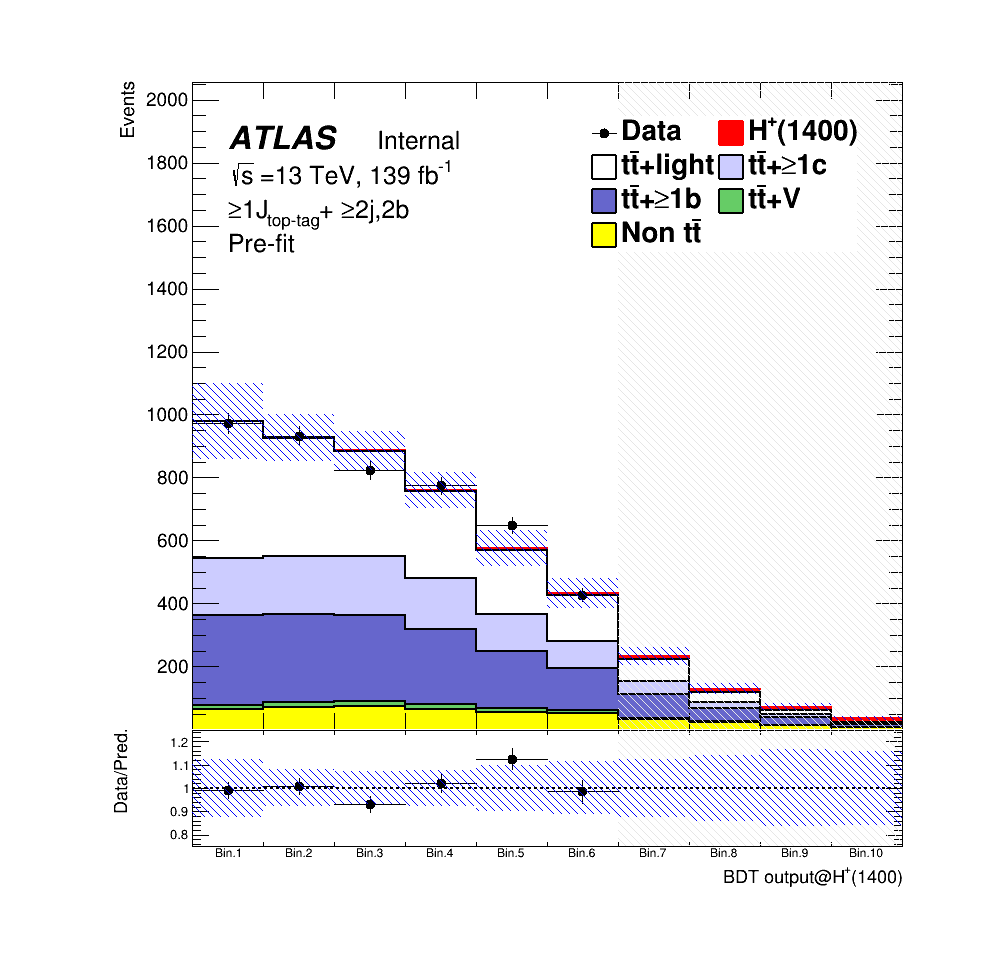
\includegraphics[width=0.50\textwidth]{images/BkgModeling/DATAOVERMC_Hp1400_Contained80_DL1r_70_bdt_Hp1400_geq1tgeq2j2b_prefit.png}
    \label{fig:BDT_Hp1400_InSR1_AfterRW}
  }
  \subfloat[] {
    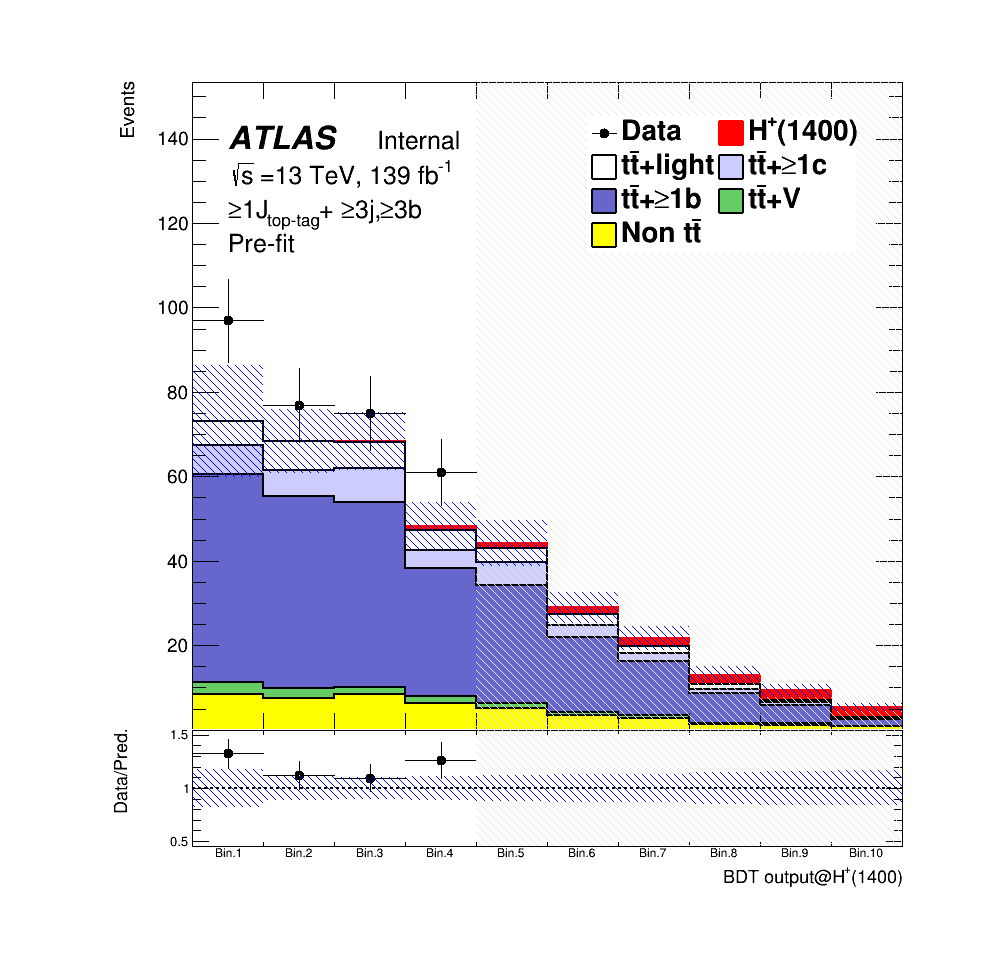
\includegraphics[width=0.50\textwidth]{images/BkgModeling/DATAOVERMC_Hp1400_Contained80_DL1r_70_bdt_Hp1400_geq1tgeq3jgeq3b_prefit.png}
    \label{fig:BDT_Hp1400_InSR2_AfterR}
  }
  \caption{Pre-fit distributions of BDT output trained using 1400 GeV $H^{+}$ in the SR1 (a) and SR2 (b) after reweighting.}
  \label{fig:DataMCComparison_bdt_Hp1000_AfterRW}
\end{figure}
\begin{figure}[H]
  \subfloat[] {
    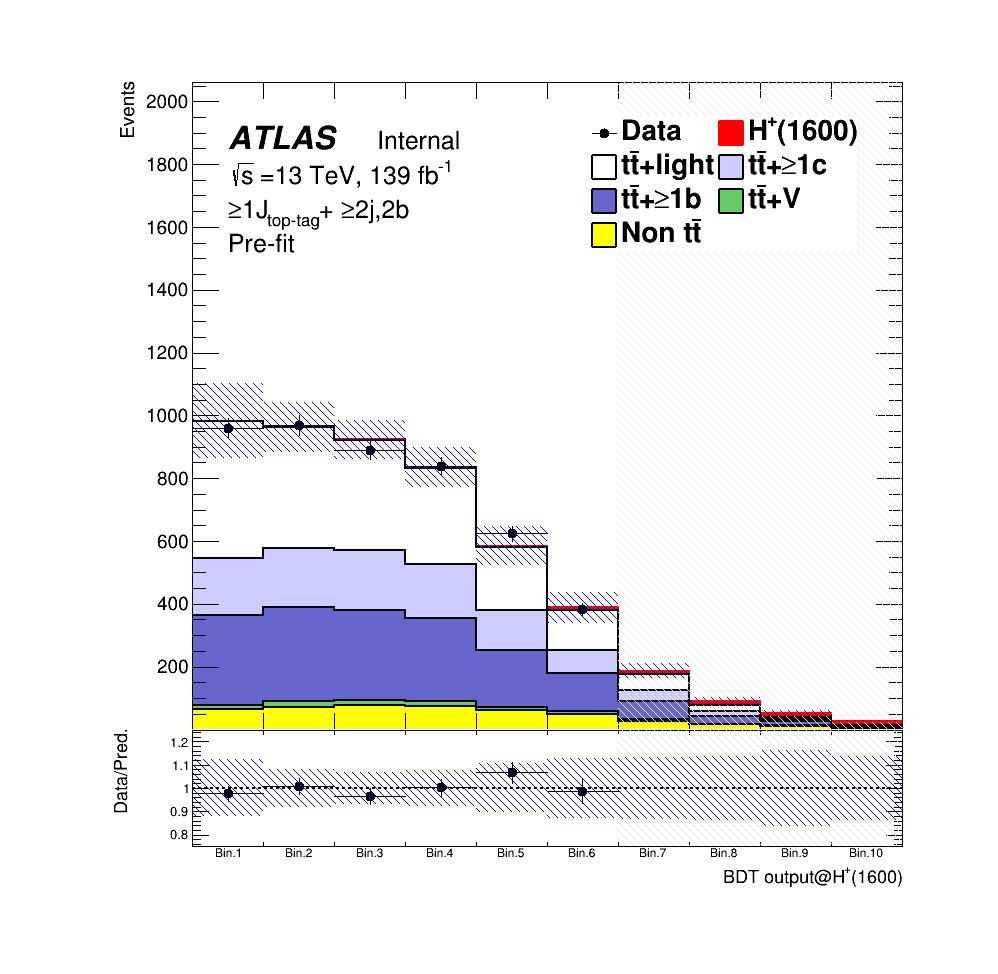
\includegraphics[width=0.50\textwidth]{images/BkgModeling/DATAOVERMC_Hp1600_Contained80_DL1r_70_bdt_Hp1600_geq1tgeq2j2b_prefit.png}
    \label{fig:BDT_Hp1600_InSR1_AfterRW}
  }
  \subfloat[] {
    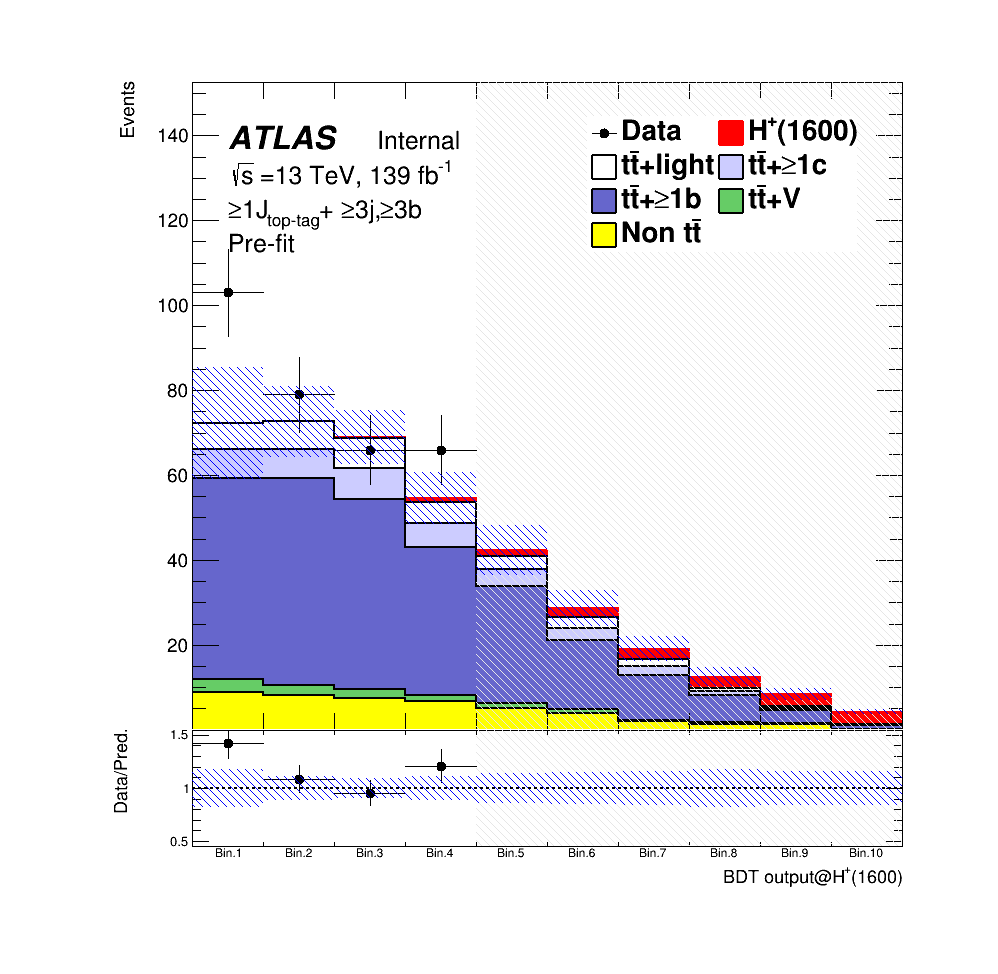
\includegraphics[width=0.50\textwidth]{images/BkgModeling/DATAOVERMC_Hp1600_Contained80_DL1r_70_bdt_Hp1600_geq1tgeq3jgeq3b_prefit.png}
    \label{fig:BDT_Hp1600_InSR2_AfterR}
  }
  \caption{Pre-fit distributions of BDT output trained using 1600 GeV $H^{+}$ in the SR1 (a) and SR2 (b) after reweighting.}
  \label{fig:DataMCComparison_bdt_Hp1600_AfterRW}
\end{figure}
\begin{figure}[H]
  \subfloat[] {
    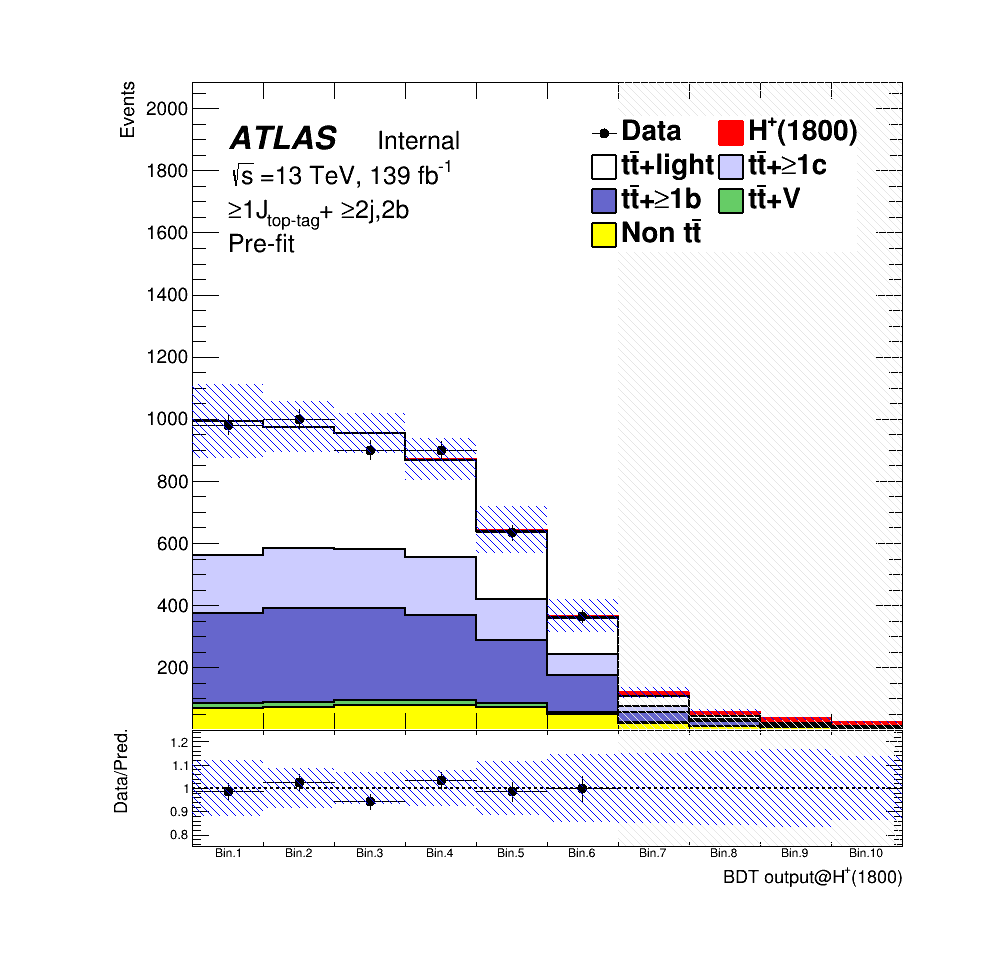
\includegraphics[width=0.50\textwidth]{images/BkgModeling/DATAOVERMC_Hp1800_Contained80_DL1r_70_bdt_Hp1800_geq1tgeq2j2b_prefit.png}
    \label{fig:BDT_Hp1800_InSR1_AfterRW}
  }
  \subfloat[] {
    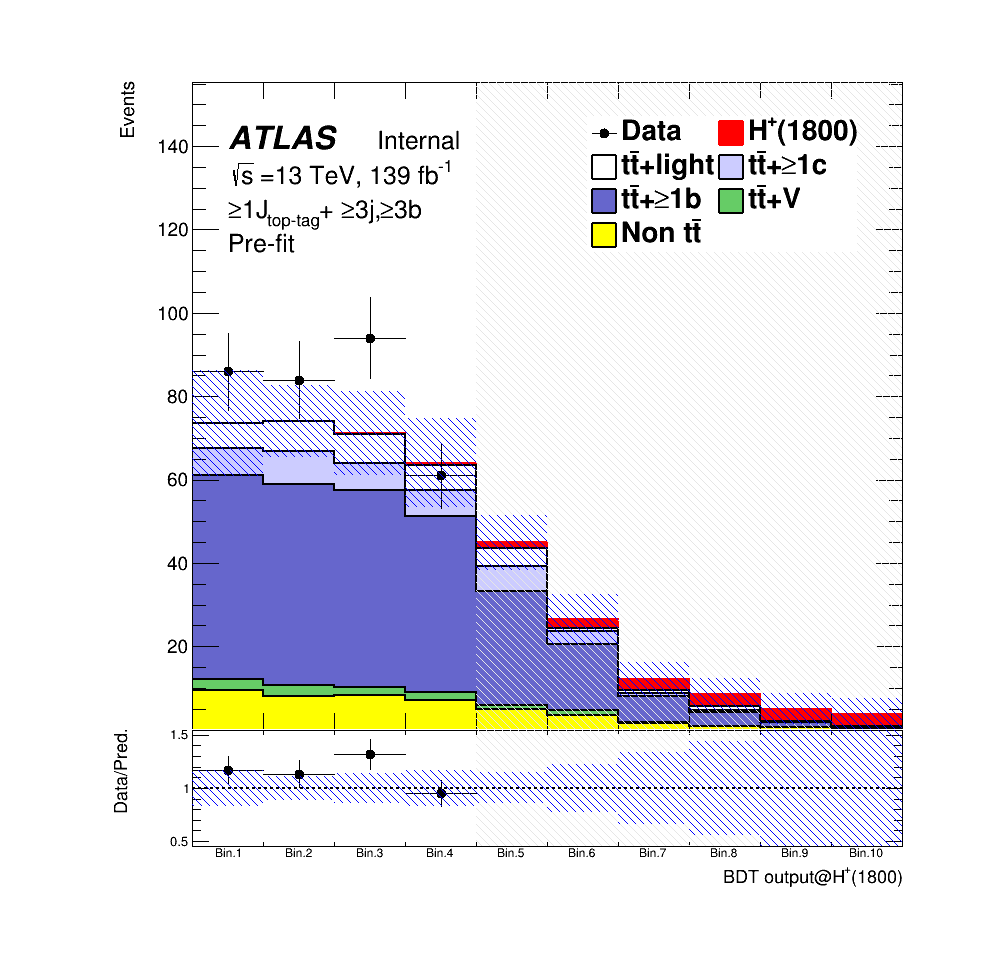
\includegraphics[width=0.50\textwidth]{images/BkgModeling/DATAOVERMC_Hp1800_Contained80_DL1r_70_bdt_Hp1800_geq1tgeq3jgeq3b_prefit.png}
    \label{fig:BDT_Hp1800_InSR2_AfterR}
  }
  \caption{Pre-fit distributions of BDT output trained using 1800 GeV $H^{+}$ in the SR1 (a) and SR2 (b) after reweighting.}
  \label{fig:DataMCComparison_bdt_Hp1800_AfterRW}
\end{figure}
\begin{figure}[H]
  \subfloat[] {
    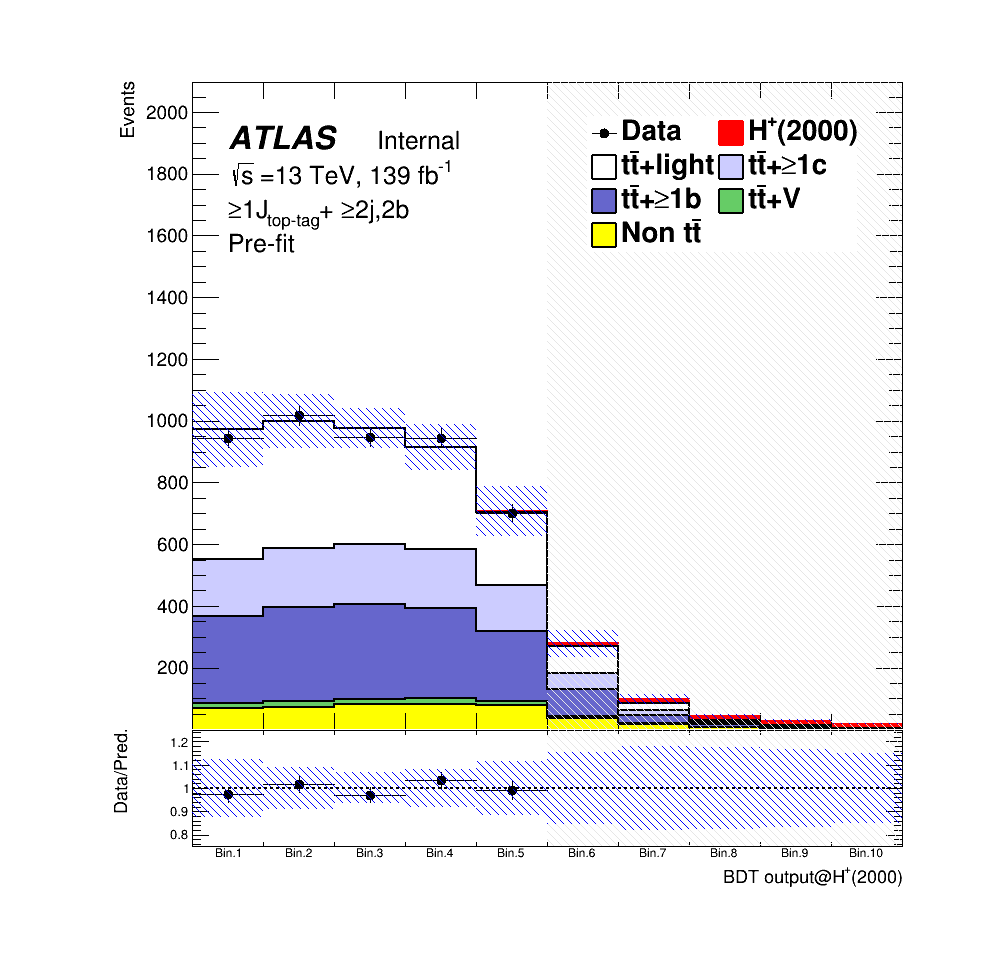
\includegraphics[width=0.50\textwidth]{images/BkgModeling/DATAOVERMC_Hp2000_Contained80_DL1r_70_bdt_Hp2000_geq1tgeq2j2b_prefit.png}
    \label{fig:BDT_Hp2000_InSR1_AfterRW}
  }
  \subfloat[] {
    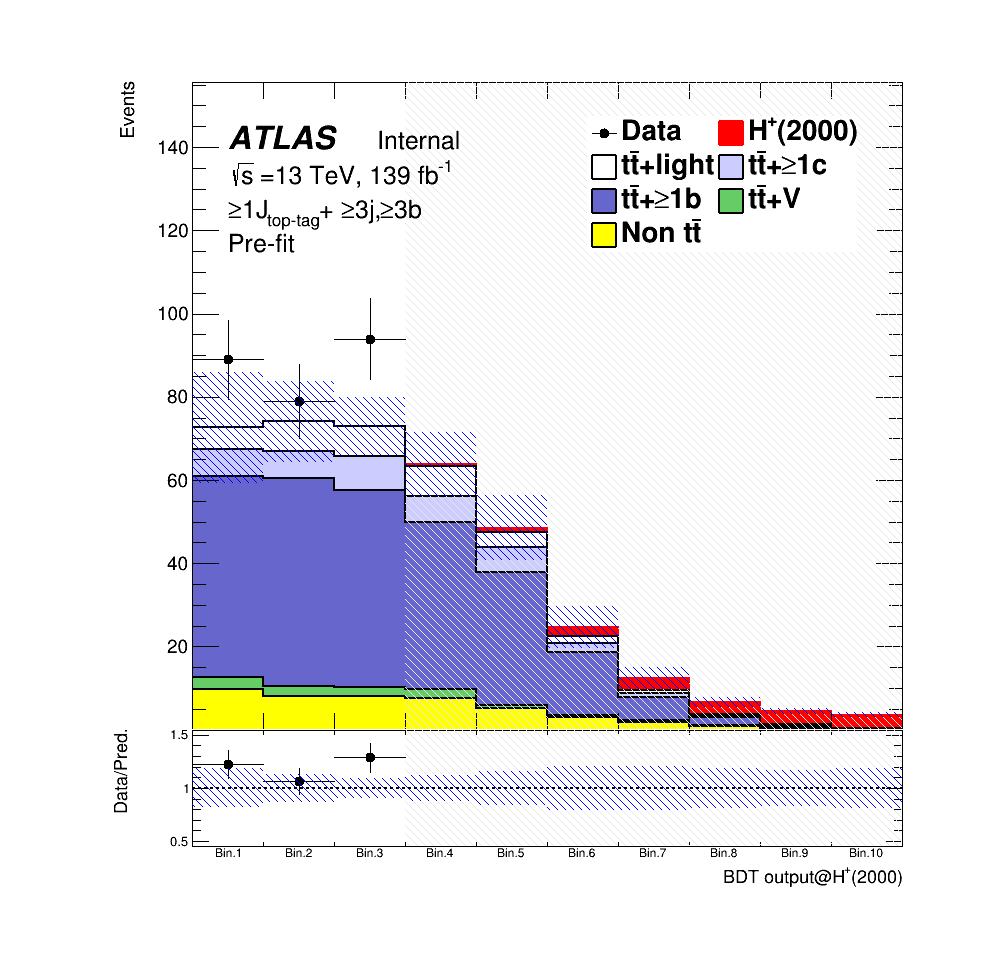
\includegraphics[width=0.50\textwidth]{images/BkgModeling/DATAOVERMC_Hp2000_Contained80_DL1r_70_bdt_Hp2000_geq1tgeq3jgeq3b_prefit.png}
    \label{fig:BDT_Hp2000_InSR2_AfterR}
  }
  \caption{Pre-fit distributions of BDT output trained using 2000 GeV $H^{+}$ in the SR1 (a) and SR2 (b) after reweighting.}
  \label{fig:DataMCComparison_bdt_Hp2000_AfterRW}
\end{figure}
\begin{figure}[H]
  \subfloat[] {
    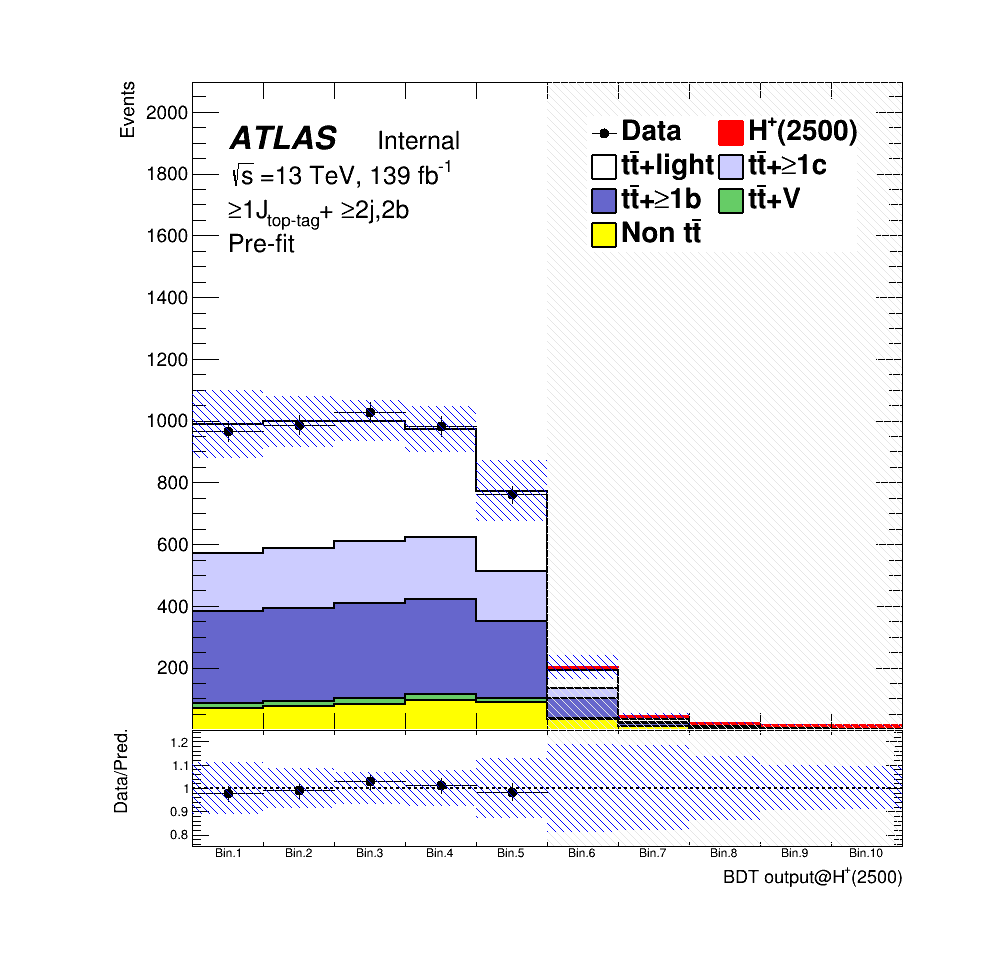
\includegraphics[width=0.50\textwidth]{images/BkgModeling/DATAOVERMC_Hp2500_Contained80_DL1r_70_bdt_Hp2500_geq1tgeq2j2b_prefit.png}
    \label{fig:BDT_Hp2500_InSR1_AfterRW}
  }
  \subfloat[] {
    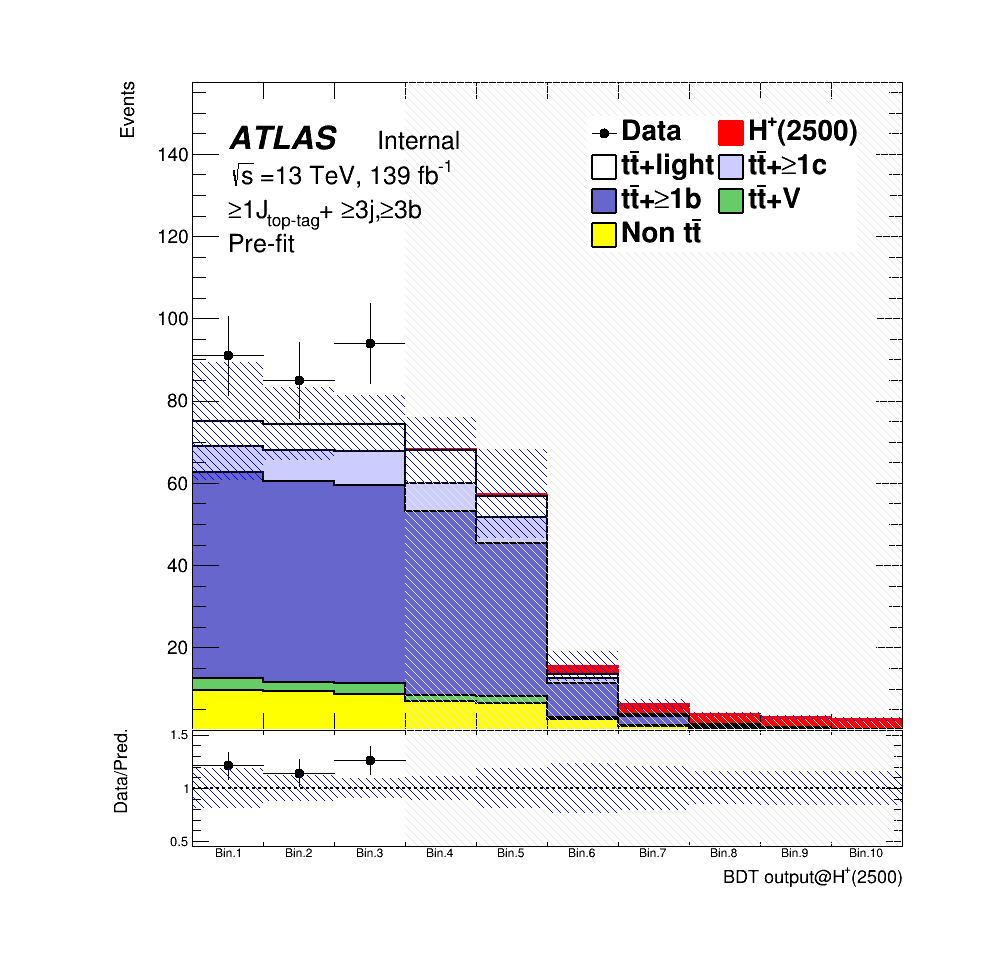
\includegraphics[width=0.50\textwidth]{images/BkgModeling/DATAOVERMC_Hp2500_Contained80_DL1r_70_bdt_Hp2500_geq1tgeq3jgeq3b_prefit.png}
    \label{fig:BDT_Hp2500_InSR2_AfterR}
  }
  \caption{Pre-fit distributions of BDT output trained using 2500 GeV $H^{+}$ in the SR1 (a) and SR2 (b) after reweighting.}
  \label{fig:DataMCComparison_bdt_Hp2500_AfterRW}
\end{figure}
\begin{figure}[H]
  \subfloat[] {
    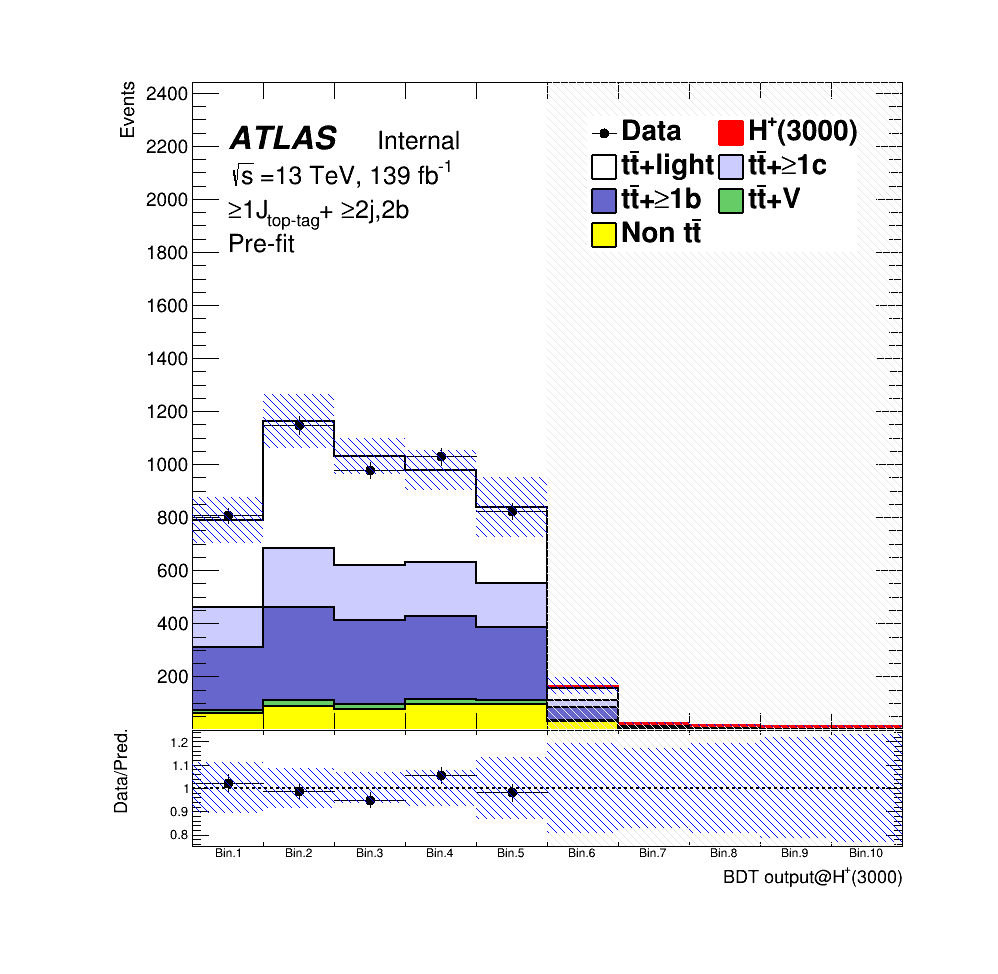
\includegraphics[width=0.50\textwidth]{images/BkgModeling/DATAOVERMC_Hp3000_Contained80_DL1r_70_bdt_Hp3000_geq1tgeq2j2b_prefit.png}
    \label{fig:BDT_Hp3000_InSR1_AfterRW}
  }
  \subfloat[] {
    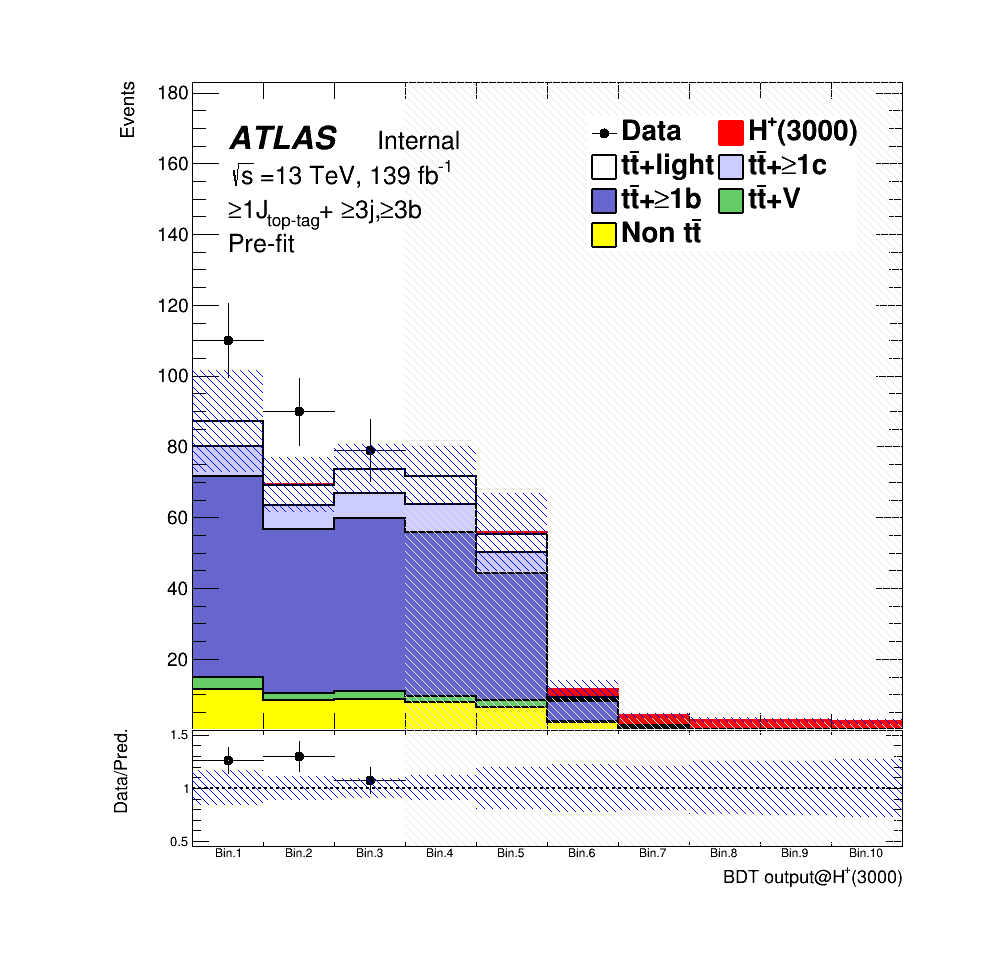
\includegraphics[width=0.50\textwidth]{images/BkgModeling/DATAOVERMC_Hp3000_Contained80_DL1r_70_bdt_Hp3000_geq1tgeq3jgeq3b_prefit.png}
    \label{fig:BDT_Hp3000_InSR2_AfterR}
  }
  \caption{Pre-fit distributions of BDT output trained using 3000 GeV $H^{+}$ in the SR1 (a) and SR2 (b) after reweighting.}
  \label{fig:DataMCComparison_bdt_Hp3000_AfterRW}
\end{figure}